%\documentclass[final,journal,letterpaper]{IEEEtran}
\documentclass[prodmode,acmtecs]{acmsmall}

\usepackage{subfigure}
\usepackage{cite}
\usepackage{amsmath}
\usepackage{amsfonts}
\usepackage{amssymb}
\usepackage{graphicx}
\usepackage{url}
\usepackage{balance}
\usepackage{float}
\usepackage{threeparttable}

\usepackage[T1]{fontenc}
\usepackage[latin9]{inputenc}
\usepackage{textcomp}
\usepackage{mathrsfs}
%\usepackage{amsthm}

\usepackage{mathptmx}
\usepackage[scaled=.90]{helvet}
\usepackage{courier}

\usepackage{color}

\usepackage{listings}
\usepackage[ruled]{algorithm2e}



\lstset{
   language=C,
   basicstyle=\small,
   keywordstyle=\bfseries,
   identifierstyle=\ttfamily,
   stringstyle=\ttfamily,
   numbers=left,
   numberstyle=\tiny,
   stepnumber=1,
   numbersep=-5pt,
   showstringspaces=false
%   frame=single %trbl%
}

\usepackage[normalem]{ulem}

%------------------------------------------------------------------------------
\newcommand{\figR}[1]{Fig.~\ref{fig:#1}}
\newcommand{\figLC}[2]{
        \caption{#2}
        \label{fig:#1}
        %\vspace{-10pt}
}
\newcommand{\secL}[1]{\label{sec:#1}}
\newcommand{\secR}[1]{Sec.~\ref{sec:#1}}

\newcommand{\defL}[1]{\label{def:#1}}
\newcommand{\defR}[1]{Def.~\ref{def:#1}}


\newcommand{\etal}{\emph{et al.}}
\newcommand{\eg}{\emph{e.g.}}
\newcommand{\ie}{\emph{i.e.}}
\newcommand{\etc}{\emph{etc.}}

\newcommand{\comment}[1]{\textcolor{red}{\bf #1}}
%\newcommand\comment[1]{} % When you enable this lines, all the notes will disappear


%\renewcommand{\baselinestretch}{0.98}\normalsize
%------------------------------------------------------------------------------
%\makeatletter
%%%%%%%%%%%%%%%%%%%%%%%%%%%%%%% Textclass specific LaTeX commands.
%\theoremstyle{plain}
%\newtheorem{thm}{\protect\theoremname}
%\theoremstyle{definition}
%\newtheorem{defn}{\protect\definitionname}
%\theoremstyle{remark}
%\newtheorem{rem}{\protect\remarkname}


%\usepackage{babel}
\providecommand{\definitionname}{Definition}
\providecommand{\remarkname}{Remark}
\providecommand{\theoremname}{Theorem}

\begin{document}
% Page heads
\markboth{V. Catania et al.}{Parameter Space Representation of Pareto Front to
Explore Hardware-Software Dependencies}


\title{Parameter Space Representation of Pareto Front to
Explore Hardware-Software Dependencies}
\author{VINCENZO CATANIA
\affil{University of Catania}
ANDREA ARALDO
\affil{University of Catania}
DAVIDE PATTI
\affil{University of Catania}
}

%\maketitle
\begin{abstract}
Embedded Systems Design requires conflicting objectives to be
optimized with an appropriate choice of hardware/software parameters. A simulation campaign guides the design in finding the best trade-offs, but, due to the big number of possible configurations, it is unfeasible to simulate all of them. For these reason Design Space Exploration (DSE) algorithms aim at finding near-optimal system configurations, only simulating a subset of them.

In this work we present PS, a new multiobjective exploration algorithm. The basic idea is to recognize \emph{interesting}, i.e. regions of the configuration space that are proving to provide better configurations w.r.t. other ones. PS evaluates more configurations in interesting regions while exploring less thoroughly the rest of the configuration space. After a detailed formal description
of the algorithm and the underlying concepts, we show a hardware/software
exploration case study. Qualitative and quantitative comparisons of PS
against a well-know multiobjective genetic approach demonstrate that,
while not outperforming it in terms of dominance, the proposed
approach can trade the uniformity and granularity qualities of the
solutions found for obtaining larger Pareto sets, thus representing a
further choice for designer when objective constrains allow it.
\end{abstract}

\category{D.2.2}{Design Tools and Techniques}{}

\terms{Design, Algorithms, Performance}

\keywords{DSE, MultiObjective Optimization, Genetic Algorithms}

\acmformat{Vincenzo Catania, Andrea Araldo and Davide Patti, 2014. Parameter Space Representation of Pareto Front to
Explore Hardware-Software Dependencies.}

\begin{bottomstuff}
Author's addresses: V. Catania, DIEEI University of Catania;
A. Araldo, DIEEI University of Catania;
D. Patti, DIEEI University of Catania.
\end{bottomstuff}

\maketitle
%------------------------------------------------------------------------------

\section{Introduction and Motivation}

The design of an embedded system requires different conflicting
objectives (energy consumption, performance, area) to be fulfilled.
Several factors are involved in this goal and real cases show how
often no analytical results are known to predict the relation between
system configurations and objectives. In such cases an high level
system simulation is often the only way to have a picture of how system
parameters impact on the objectives.  A key problem is that the size
of the design space to be simulated grows with the product of
cardinalities of each parameter, easily resulting in an untractable number
of simulations. In these cases a ``Design Space
Exploration'' strategy is required, i.e. a methodology to evaluate
only a small subset of all possible configurations while maintaining a
good level of efficiency and accuracy~\cite{surviving_soc}.

The final result of a design space exploration is a subset of the
configurations called Pareto Set (\cite{pareto}) (See also Definition
\ref{pers02.def:Pareto-set}. It represents the trade-offs between
objectives, so that for each of configuration of the Pareto Set there is no
other configuration performing better for all the objectives
considered. Once these few promising configurations have been obtained, a
subsequent step of the design flow can eventually afford a more
accurate low level simulation.

In this work we present PS, a multiobjective design exploration
strategy that introduces the concept of Parameter Space Representation
of Pareto Set. The main idea is focusing on the ``innovation''
introduced in the Pareto sets and then accordingly distribuiting the
exploration effort in regions created in the multidimensional space of
system parameters.

Many different design space exploration algorithms have been proposed
in literature.  The motivations of an exploration
algorithm are rather heuristic, have some form of arbitrariness and,
to a large extend, intuition lies behind them.

Some exploration strategies assume some kind of ``knowledge'' about
the system parameters, their meaning and impact on design objectives.
The ``Dependency analysis'' proposed in \cite{givargis_tvlsi02}, is meant
to take advantage of the dependency among the parameters in a multiobjective
optimization problem.  With this a-priori knowledge, the designer can construct a
``dependency graph'' and recognize clusters, i.e. subsets of strongly
dependency-connected parameters. Each cluster is exhaustively evaluated
and its ``local Pareto set'' is found. Then, all local Pareto sets
are merged. Doing this way, a ``sum'' of local exhaustive evaluations
are performed instead of an exhaustive evaluation of all the possible
configurations. Some problems arise: i) In real scenarios, it may
be very difficult to recognize really independent clusters of parameters,
because there may be interdependencies among a very large number of
parameters. This may lead to the need of an exhaustive search through
almost all the possible configurations. ii) A designer may not have
a precise and complete picture of the dependencies among parameters;
for this reason the need of ``automated approaches for computing interdependencies'' is declared in the same paper. 
These drawbacks are not present in our contribution. The algorithm presented
here is also meant to take advantage of dependency but is not directly
based on dependency itself, but rather it ``catches'' dependencies
in terms of ``interesting or uninteresting regions''; as a consequence
no a-priori knowledge of dependencies is required as they are discovered
during exploration. Moreover, recognizing regions offers the capability
to capture local dependencies,  i.e. dependencies that
emerge only if parameter values are bounded to certain ranges.


Abraham, Rau and Schreiber proposed in \cite{santosh_hptr00} to decompose
the system to be evaluated into components that interact minimally
with each other. Pareto sets for each component are found and, provided
that ``monotonicity'' exists, the complete Pareto set is computed
merging the component Pareto sets. Roughly speaking (see section 4
of the same paper for more details), monotonicity property guarantees
that the best system can be obtained as a composition of the best
components. This approach would perfectly work if all the components
were perfectly isolated, i.e., if there were no dependencies among
different components (in a sense similar (but not necesarily equal)
to the one of Dependency analisys). But real scenarios seldom if ever
expose monotonicity property. This leads to some ``inaccuracies''
(as stated in section 4.6.1 of the same paper).

Other approaches take into account the concept of ``sensitivity''.
The sensitivity of an objective with the respect to a parameter is
a measure of how much the objective varies when varying that parameter.
A ``sensitivity analysis'' was used in \cite{fornaciari_codes01} in an optimization
problem with only one objective (the power-delay product of an electronic
device). This method was extended in \cite{palesi_iwsoc02} to a multiobjective
optimization. In that work the sensitivity of objectives with
the respect to each parameter is measured, and parameters are ordered
on the base on these sensitivity measures. Then, a first Pareto set
is obtained varying the first parameter, having fixed to arbitrary
values all other parameters. The Pareto set is then refined varying,
in a similar way, the other parameters, one by one. Experimental results
(see section 4.2 of the same work) show that this method is not of
good ``quality'' (as broadly defined in the introduction). The reason
can be found in the very limited and rigid exploration of the parameter
space: after computing the first Pareto set, there are no more chances
to consider configurations with values of the first parameter other
than the ones assumed in the first Pareto set calculation. Similar
limitations are imposed after computing the second Pareto set, the
third and so on. It is worth noticing that this approach can not capture
``local sensitivity'' (this drawback will be called ``local sensitivity
limitation''), i.e. the objectives may be more sensitive to some
ranges of a parameter and less sensitive to other ranges of the same
parameter. Moreover it can not capture ``combined sensitivity''
(``combined sensitivity limitation''), i.e. the objectives may be
more sensitive to a range of a parameter $p_{1}$, only when other
parameters are within certain ranges, and less sensitive to the same
range of parameter $p_{1}$ when the other parameters are not within
those ranges. Therefore, in the method we propose, we do not use the
sensitivity directly, but we use the concept of innovation (that can
be considered, at least weakly related to the sensitivity). We do
not measure innovation of a parameter (as done for the sensitivity),
but rather we measure the innovation of a ``region'' of parameter
space, in order to overcome both the ``local sensitivity limitation''
and the ``combined sensitivity limitation'' stated above for the
sensitivity analysis.

Many studies focus on genetic approaches to resolve multiobjective
optimization problems (\cite{coello_easmop} and others). Genetic approaches
have many advantages: they have proved good quality (as broadly defined
in the introduction), they are customizable, they are very general
and require no a-priori knowledge to the designer.  The strong
point of genetic approaches can be summarized saying that they consist
in a broad exploration (the mutation permits to make the exploration
not rigidly restricted to limited parts of parameter space), although
this exploration is not random but is guided by the performances of
the already evaluated configurations. Therefore, the exploration is
neither too much constrained nor too much random. We claim that the
approach presented in this paper has most of the benefits of the genetic
approaches, although the rational is completely different.

The paper is organized as follows: in
Section~\ref{sec:statement_of_the_problem} we formally introduce the
main concepts and the definitions required to apply the proposed strategy. Next in
Section~\ref{sec:algorithm} we present the PS algorithm in detail.
Finally in Section~\ref{sec:ee} we show a case study involving the
exploration of the hardware/software parameters of a VLIW
architecture, performing a qualitative and quantitative comparison of
PS agains the state-of-art of multiobjective genetic based approaches.


\section{Underlying concepts and theoretical formulation}
\secL{statement_of_the_problem}

In this section we provide the concepts and the formal
definitions that we will use later to express PS, the algorithm we
propose.  First, we give the definitions of Pareto set and Pareto
front that lie on the basis of Design Space Exploration.
Then, we sketch the fundamental idea behind our algorithm. Finally, we
provide a formal definition of the regions, of their properties and of
the operations that will be performed on them by the algorithm.

In this section and the following one, we will deliberately keep our formulation as general as possible, even if the focus of this paper is the embedded system design space exploration. The goal is to make the generality of PS emerge. We argue that it is a strong point for PS, as for genetic algorithms, since (i) it permits to apply it to a wide range of different problems and (ii) it can be effectually used when the embedded system design is particularly challenging and no much a-priori knowledge is available to the designer. As already pointed in \secL{related_work}, the generality of genetic algorithms has made them widely deployed with respect to the other approaches.
Thanks to the generality of PS, we will not need to modify or adapt it in order to apply it to the case of embedded system design, as we will show in \secL{ee}. On the one hand, this legitimate our choice of keeping formulation general. On the other hand, more importantly, this confirms the capability of PS to automatically adapt to the problem under investigation, without any explicit intervention or knowledge of the designer, required, on the contrary, by~\cite{givargis_tvlsi02,santosh_hptr00,dellnitz2005covering} .

\subsection{Pareto set and Pareto front}
\secL{pareto}

Let $S$ be a parameterized system with $n$ parameters. The generic
parameter $p_i, \ i \in \{1,2,\ldots,n\}$ can take any value in
the set $V_i$. A {\em configuration} $\mathbf{c}$ of the system
$S$ is a $n$-tuple $\langle v_1,v_2,\ldots,v_n \rangle$ in which
$v_i \in V_i$ is the value fixed for the parameter $p_i$. The {\em
configuration space} (or {\em design space}) of $S$ [which we will
indicate as $\mathcal{C}(S)$] is the complete range of possible
configurations [$\mathcal{C}(S) = V_1 \times V_2 \times \ldots
\times V_n$]. Naturally, not all the configurations of
$\mathcal{C}(S)$ can really be mapped on $S$, but only a subset 
is feasible. We call this subset {\em
feasible configuration space} of $S$ and indicate it as
$\mathcal{C}^*(S)$].

Let $m$ be the number of objectives to be optimized (e.g. power,
cost, performance, etc.). An {\em evaluation function}
$E:\mathcal{C}^*(S)\times \mathcal{B} \longrightarrow \Re^m$ associates each feasible configuration of $S$ to
an $m$-tuple of values corresponding to the objectives when any application belonging to the set of benchmarks
$\mathcal{B}$ is executed.

Given a system $S$, an application $b \in \mathcal{B}$ and two
configurations $\mathbf{c}', \mathbf{c}'' \in \mathcal{C}^*(S)$,
$\mathbf{c}'$ is said to {\em dominate} (or {\em eclipse})
$\mathbf{c}''$, if, given $\mathbf{o}'=E(\mathbf{c}', b)$ and
$\mathbf{o}''=E(\mathbf{c}'', b)$, it results that $\mathbf{o}'
\leq \mathbf{o}''$ and $\mathbf{o}' \neq \mathbf{o}''$, where
vector comparisons are interpreted component-wise and are true
only if all of the individual comparisons are true ($o'_i \leq
o''_i \ \forall \ i = 1,2,\ldots,m$). To indicate that 
$\mathbf{c}'$ dominates $\mathbf{c}''$, we use the notation
$\mathbf{c}' \succ \mathbf{c}''$.

\begin{definition}[Pareto set and Pareto front]
\defL{pareto-set}
The {\em Pareto-optimal set} of $S$ (or, shortly, Pareto-set) for the application $b$ is the
set:
\[ \mathcal{P}(S,b) = \left\{ \mathbf{c} \in \mathcal{C}^*(S) \ | \nexists \ \mathbf{c}' \in \mathcal{C}^*(S), \mathbf{c}' \succ \mathbf{c} \right\} \]
\end{definition}
that is, the set of configurations $\mathbf{c} \in
\mathcal{C}^*(S)$ not dominated by any other configuration.
The configurations belonging to the Pareto-optimal set are called \emph{Pareto-optimal configurations}, while the {\em Pareto-optimal front} (or, shortly, Pareto-front) is their image, i.e. the set:
\[ \mathcal{P}_{F}(S,b) = \{ \mathbf{o} | \mathbf{o} = E(\mathbf{c},b), \mathbf{c} \in \mathcal{P}(S,b) \} \]

Another fundamental concept, which adds further complexity to the
problem of multiobjective design space exploration, is the following

\begin{definition}[Parameter dependencies]
\defL{dependency}
A parameter $x$ is said to be dependent on another parameter $y$ if
the optimal value of $y$, i.e. the $x_{opt}$ which optimizes the
objectives is dependent upon the current value of $y$. 
\end{definition}
Note that when this happens, we cannot make any safe assumption on the
``meaning'' of $a$ in order to intuitively choose an appropriate
value. 

The aim of a Design Space Exploration (DSE) strategy is to give a
good approximation of the Pareto-optimal set for a system $S$ and an
application $b$, simulating as few configurations as possible.

%----------------------------------------------------------------

As we will show later, at each iteration, PS calculates an approximation $\mathscr{P}_i$ of the Pareto-set that approaches it as iterations go on. The image of $\mathscr{P}_i$ is an approximation of the Pareto-front.
The simulation effort is distributed more on the regions that provide configurations in $\mathscr{P}_i$ which introduce more \emph{innovation}, i.e. whose image in the objective space is more distant, thus ``more different'', from the previous Pareto-front approximation point.




% A PROPOSITO DI QUESTO DUBBIO:
%\comment{AA: Mi sembra solo un cambio di notazione. DP: c'era un On the contrary troppo aggressivio, ho cercato di alleggerire la cosa, ma dai un'occhiata }
% HO CANCELLATO TUTTA QUESTA PARTE.
% For each point of the Pareto front we can imagine the corresponding configuration as a point of $P_{1}\times\dots\times P_{n}$ space. We will also refer to these points as ``parameter space representation'' of the Pareto front. \figR{psos} shows the relation between the objective space (containing the Pareto front) and its parameter space representation. In particular in this work we are interested in the relation between the evolution of the points in the two spaces, e.g. how some properties of the Pareto front points can reflect some features of the corresponding points in the parameter space.

\begin{figure}[t]
\figLC{psos}{Relation between Pareto-set and Pareto front.}
\center
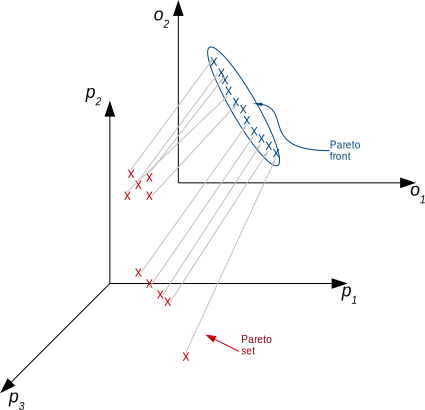
\includegraphics[width=0.5\columnwidth]{img/Pareto_set_and_front}
\end{figure}

\subsection{Sketch of the Idea}
\secL{sketch}

In the design process, there are often a lot of ``local decisions'' in
which the designer can take advantage of well-known results or
heuristics. For example, if we consider a highly parallel
computer architecture in a configuration with very few registers, it is
well-known that increasing the number of ALUs does not bring tangible
better performances but only cause an increase in area occupation. An
intelligent exploration algorithm would not waste time evaluating
configurations with many ALUs and few registers. If $p_{1}$ is the
parameter ``number of registers'' and $p_{2}$ is the parameter
``number of ALUs'', we can say that the region:
\[
R=\left\{ \left.\left(v_{1},v_{2}\right)\in P_{1}\times P_{2}\right|v_{1}<s_{1},v_{2}>s_{2}\right\} 
\]
 (where $s_{1}$ and $s_{2}$ are some threshold values) is \emph{uninteresting}. This clearly shows that there are cases when, if a parameter lies in
a certain range, there are ranges of the other one that are not worth being explored. Intuitively, the cartesian product of these ranges is an \emph{uninteresting region}.

The problem is that, in complex scenarios, not all the relations of this
kind are known in advance. Some dependency may be hidden
to the designer.
Therefore, as stated in \secR{Related-work},
setting up an exploration trying to take into account as much dependencies
as possible is a hard task that is destined to be incompletely
accomplished. We need a methodology to ``automatically'' recognize
interesting or uninteresting regions without requiring a priori knowledge
to the designer, that is what our algorithm does.

We also consider, in measuring how much interesting a region is, the
\emph{innovation} that it adds. If, during a design space exploration,
a Pareto front approximation is temporarily calculated, adding a new Pareto front
point near to the previous ones is not a considerable innovation,
because the way it fulfills the objectives is similar to the other
already evaluated configurations. On the contrary, adding a new Pareto
front point that is distant from previous ones is remarkable,
since it let the experimenter discover potential performance that have not yet considered before.
At each iteration, PS ``zooms in'' the most interesting regions while ``zooming out'' from the rest of configuration space. In order to implement this behavior algorithmically, at each iteration PS assigns the same number $N$ of simulations to each region. If a region $R$ is interesting, it is split in $k$ sub-regions before the next iteration starts. Therefore, in the next iteration, $N$ simulations are assigned to each sub-region. As a result, we are populating the original region $R$ with $k\cdot N$ simulations. On the contrary, uninteresting regions are merged, so that each one will receive less effort in the next iteration. In other words, ares of the configuration space that are more promising are split in small sub-regions, while the other ones are blended in big regions. As illustrated in \figR{small_and_big}, assigning $N$ simulations to each region makes small ones well populated while bigger ones sparsely explored.


	\begin{figure}[t]
	\center
	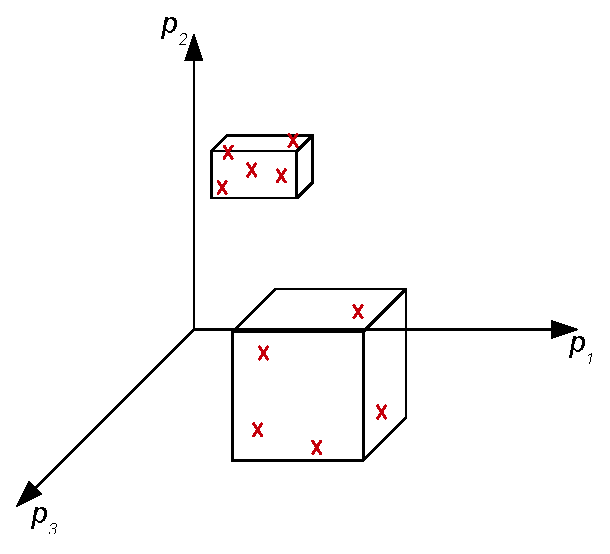
\includegraphics[width=0.5\columnwidth]{img/small_and_big}
	\figLC{small_and_big}{In this example 5 configurations
	are evaluated in a small region and in a bigger region. In can be
	seen that smaller region is more crowded.}
	\end{figure}


\subsection{Formal definitions}
We start by defining the parameter interval and the concept of interval contiguity. Using these definition we construct the region and define the region contiguity. Then we define the operations of splitting and merging regions. Finally, we provide the definition of separation.

Since regions will be defined as cartesian products of parameter intervals, we need the following definition.
\begin{definition}[Parameter interval] Let $p_{i}$ be a parameter and $a_{i},b_{i}\in V_{i},a_{i}<b_{i}$.
A $p_{i}$- interval is
	\[
	\left[a_{i}..b_{i}\right]=\left[a_{i},b_{i}\right]\cap P_{i}
	\]
i.e. taking the interval $\left[a_{i}..b_{i}\right]$
is the set of values of $V_{i}$ lying in $\left[a_{i},b_{i}\right]$)
\end{definition}


	\begin{figure}[t]
		\begin{center}
			\subfigure[Examples of contiguous and non contiguous intervals.]{
				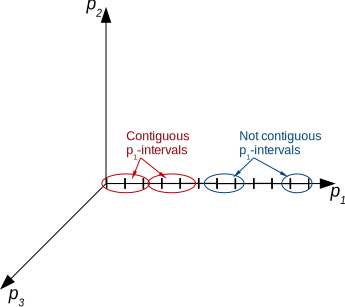
\includegraphics[width=0.45\textwidth]{img/contiguous_intervals_or_not} }
			\subfigure[Examples of regions.]{
				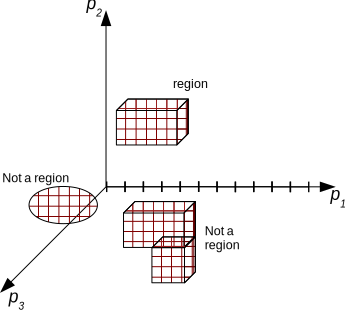
\includegraphics[width=0.45\textwidth]{img/regions} }
		    \figLC{interval_and_region}{Intervals and regions.}
		\end{center}
	\end{figure}



We consider only parameters $p_{i}$ with ordering, i.e. such
that $\forall a,b\in V_{i}$ it is possible
to say $a<b$ or $a=b$ or $a>b$. 
The following definition of interval contiguity will be the base of the concept of region contiguity, used to define merging and splitting operations.
\begin{definition}[Contiguous intervals]
\label{pers02.def:Contiguous-intervals}
Two intervals are contiguous iff they do not overlap and merging them results in a new interval. More formally, let $\left[a_{i}..b_{i}\right]$ and $\left[x_{i}..y_{i}\right]$
be two $p_{i}$-intervals. They are said to be contiguous (see \figR{interval_and_region}(a) ) iff
\begin{align}\begin{array}{l}
	\left[a_{i}..b_{i}\right]\cap\left[x_{i}..y_{i}\right]=\emptyset \mbox{      and} \\
	\left[a_{i}..b_{i}\right]\cup\left[x_{i}..y_{i}\right]$ is a $p_{i}$-
interval or $\left[x_{i}..y_{i}\right]\cup\left[a_{i}..b_{i}\right]
\end{array}\end{align}
\end{definition}

\begin{definition}[Region] 
A region is a cartesian product of parameter intervals, as illustrated in \figR{interval_and_region} (b). More formally, if $p_1,\dots,p_n$ are the parameters of the system, and $\left[ a_{i}..b_{i} \right]$ is a $p_i$-interval, a region is a set of the following form:
\[
R=\left[a_{1}..b_{1}\right]\times\dots\times\left[a_{n}..b_{n}\right]=\prod\left[a_{i}..b_{i}\right]
\]
\end{definition}

We will refer later to ``big'' and ``small'' regions. The sense
of these terms is related to the cardinality of regions.
\begin{definition}[Interval and region comparison]
A $p_{i}$-interval $\left[a_{i}..b_{i}\right]$
is said to be bigger then another $p_{i}$-interval $\left[c_{i}..d_{i}\right]$
iff 
$\left|\left[a_{i}..b_{i}\right]\right|>\left|\left[c_{i}..d_{i}\right]\right|$.
Similarly, a region $R_{1}$ is said to be \emph{bigger }then $R_{2}$, if
$\left|R_{1}\right|>\left|R_{2}\right|$
\end{definition}
Note that with $|\cdot|$ we indicate the cardinality of a set. Therefore, $\left|\left[a_{i}..b_{i}\right]\right|$ is the number of values of $V_i$ lying between $a_{i}$ and $b_{i}$ and has not to be confused with $b_i - a_i$.
Similarly $\left|R_{i}\right|$ is the number of configurations inside the region $R_i$.

As already explained, we will split interesting regions and merge uninteresting ones. The region splitting and merging operations are defined starting from the corresponding operations defined on intervals.
\begin{definition}[Splitting an interval]
\defL{splitting-a-region}
Given a $p_i$ interval $\left[a_{i}..b_{i}\right]$ with more than one element, i.e. $\left|\left[a_{i}..b_{i}\right]\right|>1$, the splitting operation produces as result two contiguous intervals $\left[a_{i}..c_{i}\right],\left[d_{i}..b_{i}\right]$
 such that
	\begin{align}
		\begin{cases}
		\left[a_{i}..c_{i}\right]\cap\left[d_{i}..b_{i}\right] & =\emptyset\\
		\left[a_{i}..c_{i}\right]\cup\left[d_{i}..b_{i}\right] & =\left[a_{i}..b_{i}\right]\\
		\left|\left[a_{i}..c_{i}\right]\right| & =\left\lceil \frac{\left|\left[a_{i}..b_{i}\right]\right|}{2}\right\rceil 
		\end{cases}
	\end{align}

We define the split operator $\psi$ as the one that, when applied to the intervals, gives the result of the split operation, i.e., in the case above, $\psi \left[a_{i}..b_{i}\right]=\lbrace \left[a_{i}..c_{i}\right],\left[d_{i}..b_{i}\right] \rbrace$.
If $\left|\left[a_{i}..b_{i}\right]\right|=1$, the interval
cannot be split and $\psi \left[a_{i}..b_{i}\right]=\left[a_{i}..b_{i}\right]$.
\end{definition}

The interval split is illustrated in \figR{split}~(a). Note that, when splitting an interval, the resulting intervals must satisfy two conditions: (i) they must be contiguous and, merging them, the initial interval must be obtained; (ii) the point in which we cut the interval is not arbitrary, but it is close to the middle.

\begin{definition}[Splitting a region]
\label{pers02.def:Splitting-a-region}
Consider a region $R=\prod\left[a_{i}..b_{i}\right]$.The split operator $\psi$ divides it into a set of sub-regions obtained splitting each $p_i$-interval and combining the resulting sub-intervals with the cartesian product, as shown in \figR{split}~(b). Formally:
	\begin{align}
		\psi(R) = \left\{ \left.\prod\left[x_{i}..y_{i}\right]\right|\left[x_{i}..y_{i}\right]\in \psi\left[a_{i}..b_{i}\right]  \right\} 
	\end{align}

\end{definition}


	\begin{figure}[t]
	    \figLC{split}{Split operations.}
		\begin{center}
			\subfigure[Splitting an interval.]{
				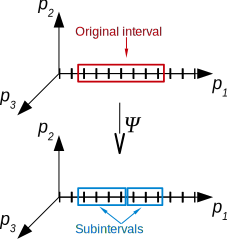
\includegraphics[width=0.30\textwidth]{img/splitting_intervals} }
			\subfigure[Splitting a region.]{
				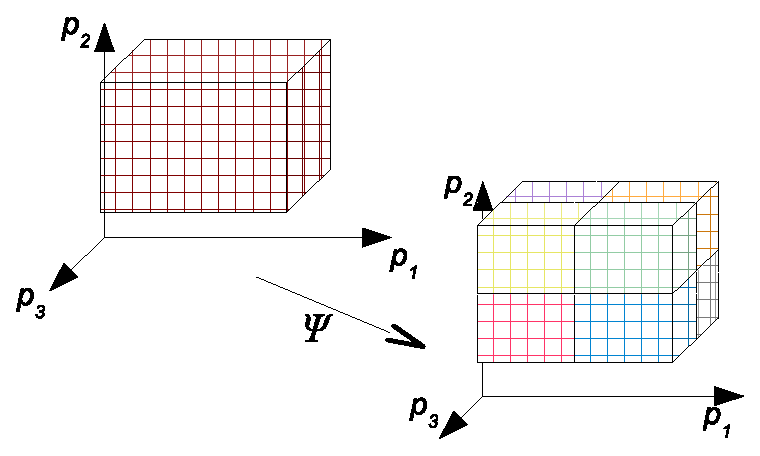
\includegraphics[width=0.60\textwidth]{img/splitting_regions} }
		\end{center}
	\end{figure}


The merging operation will be defined only on region pairs that satisfy the conditions provided in the following definition.
\begin{definition}[Contiguous regions]Let $R_{1}=\prod\left[a_{i}\dots b_{i}\right]$ and $R_{2}=\prod\left[x_{i}..y_{i}\right]$
be two regions. They are said to be contiguous iff they do not overlap and, merging them, a new region can be obtained. Formally, $R_1$ and $R_2$ are contiguous iff there exists a $j$ such that:
	\begin{align}\begin{array}{l}
		\left[a_{i}..b_{i}\right]=\left[x_{i}..y_{i}\right]$
	\mbox{ for } $i\neq j \mbox{      and} \\
		\left[a_{j}..b_{j}\right]$ and $\left[x_{j}..y_{j}\right] \mbox{ are contiguous intervals}
	\end{array}\end{align}
\noindent We call $p_j$ the \emph{contiguity parameter} for the two regions.
\end{definition}

Examples of contiguous and non contiguous regions are given in \figR{contiguous_regions}. The two regions at the top are contiguous because their union can be expressed as the cartesian product of parameter intervals, thus they can be merged to obtain a new bigger region. The same also applies to the regions on the right. On the contrary, the two regions on the left (or of the two regions at the bottom) cannot be merged. 

	\begin{figure}[t]
		\center
		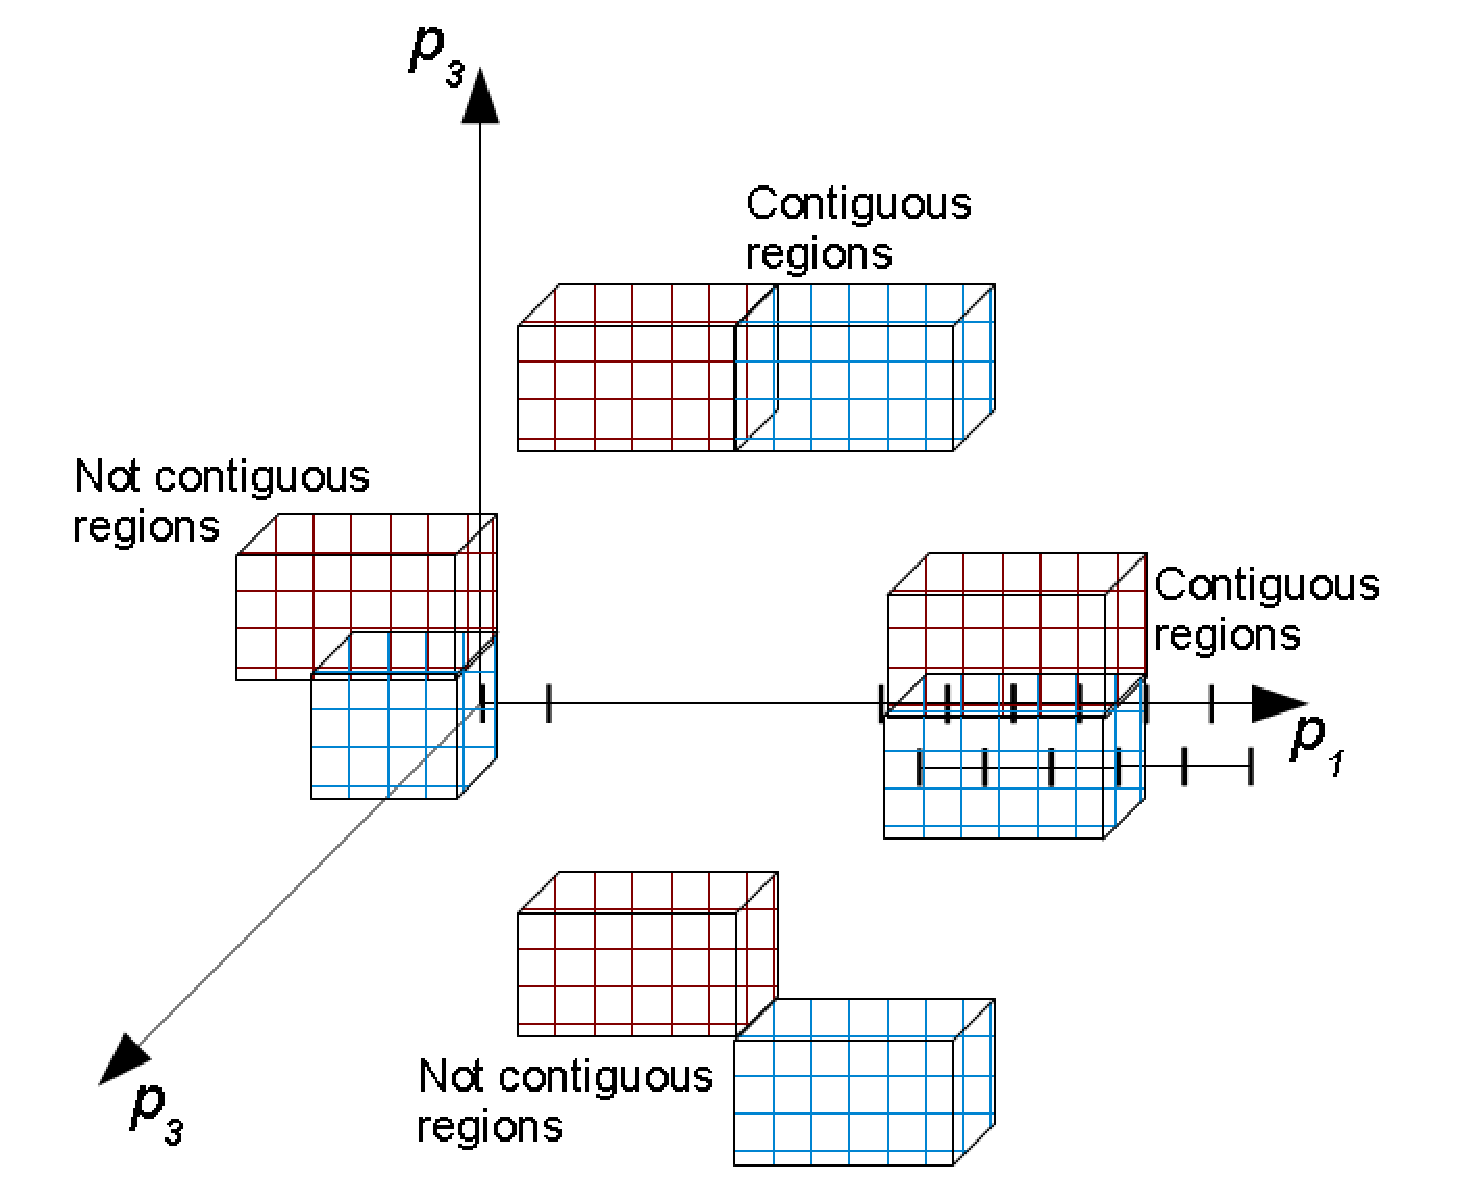
\includegraphics[width=0.8\columnwidth]{img/contiguous_regions}
		\figLC{contiguous_regions}{Contiguous and non contiguous regions.}
	\end{figure}

We now formally describe the merging operations.
\begin{definition}[Merging intervals]
Let $\left[a_{i}\dots b_{i}\right]$ and $\left[x_{i}..y_{i}\right]$ be two contiguous $p_i$-intervals. The merge operation applied to them produces a new $p_i$-interval of the following form:
	\begin{align}
		\mu	 \left( \begin{array}{l}
				\left[a_{j}..y_{j}\right] \\
				\left[x_{j}..b_{j}\right]
		     \end{array} \right)
		=\begin{cases}
			\left[a_{j}..y_{j}\right] & \mbox{ if }b_{j}<x_{j}\\
			\left[x_{j}..b_{j}\right] & \mbox{ if }y_{j}<a_{j}
		\end{cases}
	\end{align}

\end{definition}

\begin{definition}[Merging regions]
\defL{merging-regions}
Let $R_{1}=\prod\left[a_{i}\dots b_{i}\right]$ and $R_{2}=\prod\left[x_{i}..y_{i}\right]$ be two contiguous regions and let $p_j$ be the contiguity parameter. 
The merge operation $\mu$ applied to $R_1$ and $R_2$ produces a new region of the following form:
	\begin{align}
		\mu(R_1,R_2)=\prod_{i<j}\left[a_{i}..b_{i}\right]
		\times
		\mu	 \left( \begin{array}{l}
				\left[a_{j}..y_{j}\right] \\
				\left[x_{j}..b_{j}\right]
		     \end{array} \right)
		\times
		\prod_{i>j}\left[a_{i}..b_{i}\right]
	\end{align}
\end{definition}

Note that $\mu(R_{1},R_{2})$ is mathematically equivalent to $R_{1}\cup R_{2}$. However, we use the notation above to enforce the requirement that
$R_{1}$ and $R_{2}$ must be to contiguous regions.

In \secR{sketch} we observed that, in order to estimate how interesting a region is, it is crucial to understand the novelty it introduces, i.e. how distant the Pareto-optimal configurations discovered in that region are from the Pareto-optimal configuration previously discovered. The concept of distance is expressed by the operator defined in the next definition. We prefer to call it \emph{separation} rather than \emph{distance}, because usually distance denotes a commutative operator while our definition of separation is non commutative.

\begin{definition}[Separation]
\defL{separation}
Let $\mathbf{c}',\mathbf{c}''\in \mathcal{C}^*(S)$ be two configurations of the system $S$, $b\in\mathcal{B}$ a benchmark application and $\mathbf{o}',\mathbf{o}''\in \Re^m$ the representation of the configurations in the objective space, i.e. $\mathbf{o}'=E \left(\mathbf{c}', b\right)$, $\mathbf{o}''=E \left(\mathbf{c}'', b\right)$, where $E$ is the evaluation function. The separation between
$\mathbf{c}'$ and $\mathbf{c}''$ is 
	\[
	s\left(\mathbf{c}'\rightarrow\mathbf{c}''\right)=\sum_{i=1}^{m}\left|\frac{o'_{i}-o''_{i}}{o'_{i}}\right|
	\]
where $o'_i$ and $o''_i$ are the $i$-th components of $\mathbf{o}'$ and $\mathbf{o}''$, respectively.
\end{definition}

The separation between $\mathbf{c}'$ and $\mathbf{c}''$ measures how
much we must vary the image of the former to obtain the image of the latter. Note that the separation is a \emph{normalized} measure, thanks to $o'_i$ at the denominator. This is important since objectives are usually heterogeneous, e.g. delay and power consumption have different unities of measurement and different scale. If we did not use a normalized measure, in presence of objectives whose absolute values are small and other objectives with big values, the notion of distance would have been biased toward the latter.


\section{The algorithm}
\label{sec:algorithm}

The algorithm we present is iterative. Each iteration is called \emph{era}. 

Each era $era_{i}$ is characterized by 
\begin{itemize}
\item the set of regions $\mathcal{R}_{i}$ in which the parameter space
$P_{1}\times\dots\times P_{n}$ is divided
\item its Pareto set $\mathscr{P}_{i}$
\item a set $test_{i}$ of at most $K$ configurations to evaluate
\end{itemize}
$K$ is a parameter that must be set before the algorithm runs.


\subsection{Start Condition}
$\mathcal{R}_{0}=\left\{ P_{1}\times\dots\times P_{n}\right\} $,
i.e. era $0$ has only one region that is the whole parameter space.
A random set $test_{0}$ of $K$ configurations is evaluated. The
Pareto set $\mathscr{P}_{0}=\mathscr{P}\left(test_{0}\right)$ is
calculated (see def \ref{pers02.def:Pareto-set} for the definition
of the operator $\mathscr{P}_{i}$ over a set)

\subsection{Iteration Rules}

For $era_{i}$ with $i>0$ the following operations must be performed.
\begin{enumerate}
\item \label{pers02.enu:K}For each region $R\in\mathcal{R}_{i}$, a set
$test_{R,i}$ of configurations is randomly chosen in%
\footnote{Therefore the chosen configurations can only be configurations of
$R$ not yet evaluated in past eras.%
} $R\setminus\bigcup_{j=0}^{i-1}test_{j}$. The number of configurations
in $test_{R,i}$ is set to%
\footnote{This means that $\frac{K}{\left|\mathcal{R}_{i}\right|}$ configurations
are to be chosen, but if not yet evaluated configurations in $R$
are less then $\frac{K}{\left|\mathcal{R}_{i}\right|}$, all of them
are chosen%
} 
\[
\min\left(\frac{K}{\left|\mathcal{R}_{i}\right|},\left|R\setminus\bigcup_{j=1}^{i-1}test_{j}\right|\right)
\]
The set 
\[
test_{i}=\bigcup_{R\in\mathcal{R}_{i}}test_{R,i}
\]
 is defined. 
\item All configurations on $test_{i}$ are simulated.
\item The Pareto set $\mathscr{P}_{i}$ for $era_{i}$ is defined as 
\[
\mathscr{P}_{i}=\mathscr{P}\left(test_{i}\cup\mathscr{P}_{i-1}\right)
\]

\item \label{pers02.enu:novelty_score_of_a_configuration}Every point $\mathbf{p}$
of%
\footnote{The innovation score is not given to those points in $test_{i}$ that
are not in the Pareto set%
} $test_{i}\cap\mathscr{P}_{i}$ is given an \emph{innovation score
}defined as:
\[
is\left(\mathbf{p}\right)=\min\left\{ \left.s\left(\mathbf{q}\rightarrow\mathbf{o}\left(\mathbf{p}\right)\right)\right|\mathbf{q}\in\mathscr{P}_{i-1}\right\} 
\]
 (a configuration $\mathbf{p}$ is characterized by as much innovation
as more separated it is from the configurations of the previous era)\@.
\item Every region $R\in\mathcal{R}_{i}$ is given an innovation score defined
as:
\[
is\left(R\right)=\sum\left\{ \left.is\left(\mathbf{p}\right)\right|\mathbf{p}\in\mathscr{P}_{i}\cap R\right\} 
\]

\item The total innovation score for the entire era is:
\[
is_{TOT,i}=\sum_{R\in\mathcal{R}_{i}}is\left(R\right)
\]

\item The avarage innovation score for the entire era is also calculated
as:
\[
is_{av,i}=\frac{is_{TOT,i}}{\left|\mathcal{R}_{i}\right|}
\]
where $\left|\mathcal{R}_{i}\right|$ is the number of regions of
era $i$ .
\item $\mathcal{R}_{i}$ is partitioned in three subsets (their meaning
will be discussed later):

\begin{enumerate}
\item high innovation regions 
\[
\mathcal{R}_{i,h}=\left\{ \left.R\in\mathcal{R}_{i}\right|is\left(R\right)>\alpha\cdot is_{av,i-1}\right\} 
\]
 where $\alpha$ is a constant defined by the designer (for example
$\alpha=1.2$). Each $R\in\mathcal{R}_{i,h}$ is split in $\mathcal{R}^{R}$
(as stated in def \ref{pers02.def:Splitting-a-region})
\item low innovation regions 
\[
\mathcal{R}_{i,l}=\left\{ \left.R\in\mathcal{R}_{i}\right|0<is\left(R\right)\le\alpha\cdot is_{av,i-1}\right\} 
\]
They are not changed.
\item no innovation regions 
\[
\mathcal{R}_{i,n}=\left\{ \left.R\in\mathcal{R}_{i}\right|is\left(R\right)=0\right\} 
\]
\end{enumerate}

\item Disjoint couples of contiguous regions $\left(R_{1},R_{2}\right)$,
with $R_{1},R_{2}\in\mathcal{R}_{i,n}$ are selected. The set of this
couples is indicated as $\mathcal{C}$. The couples of regions are
merged:
\[
\forall\left(R_{1},R_{2}\right)\in\mathcal{C}\Rightarrow R=R_{1}+R_{2}
\]
 (see def \ref{pers02.def:Merging-regions})
\item The set of regions $\mathcal{R}_{i+1}$ for the following era is defined
as:
\[
\mathcal{R}_{i+1}=
\]
\[
=\left(\bigcup_{R\in\mathcal{R}_{i,h}}\mathcal{R}^{R}\right)\cup\mathcal{R}_{i,l}\cup
\]
\[
\cup\left(\mathcal{R}_{i,n}\setminus\bigcup_{\left(R_{1},R_{2}\right)\in\mathcal{C}}\left\{ R_{1},R_{2}\right\} \right)\cup
\]
\[
\cup\left(\bigcup_{\left(R_{1},R_{2}\right)\in\mathcal{C}}\left(R_{1}+R_{2}\right)\right)
\]

\end{enumerate}

\subsection{Termination Condition}
The algorithm terminates at step $k$ if
\[
is_{TOT,k},is_{TOT,k-1},\dots,is_{TOT,k-\beta}\le\gamma\cdot is_{TOT,k-\left(\beta-1\right)}
\]
 where $\beta$ and $\gamma$ are selected by the experimenter (see
remark \ref{rem:termination}).
\begin{rem}
\label{pers02.rem:smaller_regions}The rule \ref{pers02.enu:K} of
the iteration rules says that the smaller is a region, the more ``crowded''
it is. It means that configurations in smaller regions are evaluated
with more ``attention'' (see figure \ref{pers02.fig:small_and_big}).

\begin{figure}[h]
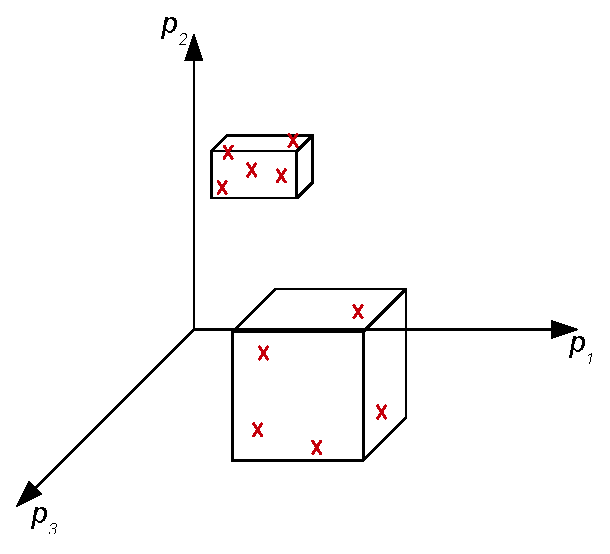
\includegraphics[width=0.9\columnwidth]{img/small_and_big}

\caption{\label{pers02.fig:small_and_big}In this example 5 configurations
are evaluated in a small region and in a bigger region. In can be
seen that smaller region is more crowded.}


\end{figure}

\end{rem}

\begin{rem}
The rule \ref{pers02.enu:novelty_score_of_a_configuration} says that
a configuration whose objectives are more ``separated'' by the previous
Pareto front, has to be taken in greater account than others. A configuration
that is very near, in the objective space, to the previous Pareto
front doesn't add a true innovation. Therefore, the innovation score
of a configuration is a measure of how much interest we have in considering
it (see figure \ref{pers02.fig:Novelty-score-of-a-config}).

\begin{figure}[h]
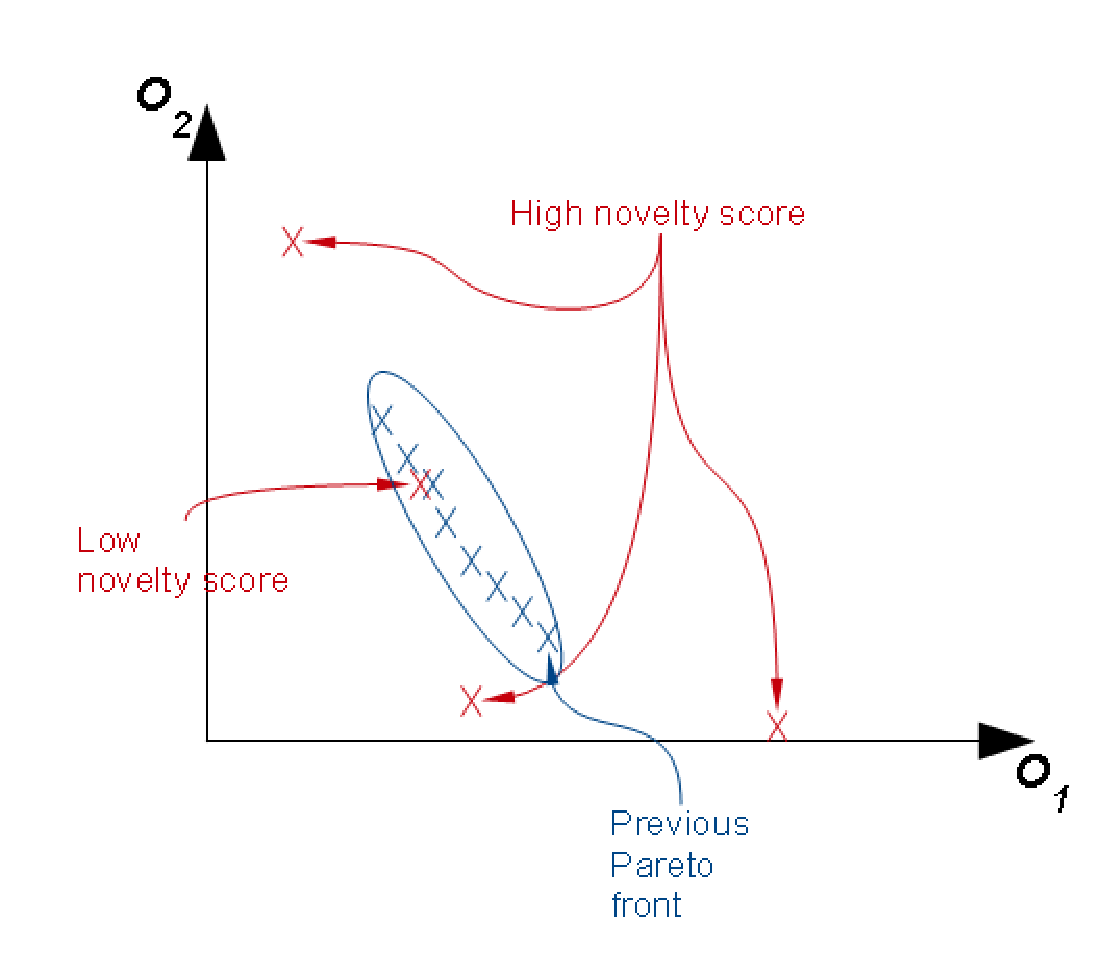
\includegraphics[width=0.9\columnwidth]{img/novelty_score}

\caption{\label{pers02.fig:Novelty-score-of-a-config}innovation score of a
configuration}


\end{figure}

\end{rem}

\begin{rem}
The innovation score of a region is a measure of how much different
are the points that it adds to Pareto Front compared to the previous
Pareto front. ``High innovation regions'' are the ones in which
more configurations are worth evaluating, because they add many points
on not yet well explored Pareto front areas. Therefore, these regions
are split in the next era (see remark \ref{pers02.rem:smaller_regions})
and more ``crowded'' by simulations. ``No innovation regions''
are the ones that have proved to add few points on Pareto fronts,
probably very near to previous Pareto front points and a Pareto front
point near to previous points is not so much interesting. Therefore
it's not worth evaluating many of their configurations and it is useful
to merge these regions, in order to less densely evaluate them.

%ULTERIORI GIUSTIFICAZIONI SULL'IMPORTANZA DI CONSIDERARE LA DIVERSITA'
%DELLE SOLUZIONI SI TROVA IN ext12.pag5 E ALTRI.

\end{rem}

\begin{rem}
\label{rem:termination}The algorithm terminates when in the last
$\beta$ iterations not a great ``amount of innovation'' has been
discovered. Therefore it is very probably that carrying on iterating
will not considerably change the Pareto front already formed. It's
not recommended to chose $\beta=1$, because it is possible that the
Pareto fronts $\mathbf{o}\left(\mathscr{P}_{k-1}\right)$ and $\mathbf{o}\left(\mathscr{P}_{k}\right)$
are not very different but next Pareto fronts could be. In other words,
it's unsafe to terminate as soon as the Pareto front doesn't change
enough between two consecutive eras, thus a strategy taking into
account the history of the Pareto fronts has been adopted in the
proposed approach.
\end{rem}
%!!! IN INGLESE E' PIU' CORRETTO DIRE: ``IT IS POSSIBLE THAT THE PARETO
%FRONTS WERE NOT VERY DIFFERENT''? (CON ``WERE'' AL POSTO DI ``ARE'')


\begin{rem}
Merging and splitting the regions are very dynamic processes. A portion
of the parameter space can be populated by a large number of small
regions in some eras, but can be covered by a small number of large
regions in next eras. This can be explained saying that, after a number
of eras of intense exploration of a portion of parameter space, this
exploration has turned to be enough thorough and so it was time for
other portions to be minutely scanned.
\end{rem}

\section{A Case Study: VLIW Hardware/Software Design Space}
\secL{ee}
Although PS has been formally introduced and described as a general
multi-objective optimization algorithm, in this work we will
embedded system design scenario,  since its properties
are the ones that suggested to the authors the concepts of Pareto-based
innovation and region scoring system.

In particular, we use a parametrized Very Long Instruction
Word (VLIW) architecture~\cite{kathail_tr00} as testbed. The philosophy
behind a VLIW system makes this a natural choice for several reasons:
\begin{itemize}
\item \emph{Multi-Objective trade-offs}: VLIW architectures allow designers
to balance power, energy and performances objectives, resulting
in extended Pareto sets which are an ideal ground for our testing
purposes focused on parameter-space representation
\item \emph{Software Compiler awareness}: code scheduling for the execution of
applications is statically obtained by the compiler which
performs code transformations ``being aware'' of the underlying hardware
configuration.  This tight hardware/software dependence makes the
VLIW scenario perfectly suitable for investigating hardly predictable
parameter interactions.
\end{itemize}

In this section, we will also briefly describe the parametrized platform used
as testbed for the experiments, the general evaluation flow along with
the high-level estimation models and applications used as benchmarks.

\subsection{Design Space: Hardware and Software Parameters}
\secL{designspace}
Conceptually, system parameters can be classified in three main categories:
\emph{processor}, \emph{memory sub-system} and \emph{compiler}. The
first two categories are directly related to the physical
implementation of the system, and thus parameters of those
classes are usually referred as ``hardware parameters''. On the other
side, all the parameters affecting the behavior of the compiler
are referred as ``software parameters'', being directly involved in
the process of generating the application executable running on the
underlying hardware.

Processor hardware parameters are directly related to the VLIW core
and include the size of the register files and the number of
functional units of each type. On the software side, a set of the most
impacting code compilation parameters has been selected.
Table~\ref{tab:param} shows the complete set of parameters included in
the design space and their possible values. The total size of the design
space, which grows with the product of parameter cardinalities, is
about $1.33 \times 10^{14}$.


As regards the class of benchmark being considered, a set of applications representative of some common
frequently running code kernels has been selected. Table~\ref{tab:bench} shows the set of applications
along with a brief description.
% IEEE table style
%\begin{table}
%	\centering
%	\caption{Benchmarks}
%	\label{tab:bench}
%	\begin{tabular}{ll}
%	\hline
%	\multicolumn{1}{c}{Benchmark} & \multicolumn{1}{c}{Application} \\
%	\hline
%	Alloca\_test & Memory array allocation test \\
%	Bmm & Matrices multiplication and elements sum \\
%	Fir\_int & Finite impulse response \\
%	Mm & Floating point matrices multiplication \\
%	Sha256 & Cryptocurrency header Hashing \\
%	Wave & Wavefront computation \\
%	\hline
%	\end{tabular}
%\end{table}


\begin{table}
	\tbl{Design Space\label{tab:param}}{
	\begin{tabular}{lll}
	\hline
	\multicolumn{1}{c}{Parameter} & \multicolumn{1}{c}{Values} & \multicolumn{1}{c}{Type}\\
	\hline
	General Purpose Registers & 16, 32, 64, 128 & HW \\
	Floating Point Registers & 16, 32, 64, 128 & HW \\
	Predicate Instructions registers & 32, 64, 128 & HW \\
	Branch Target Registers & 16, 32, 64 & HW \\
	Control Registers & 32, 64, 128 & HW \\
	\hline
	Integer Functional Units & 1, 2, 3, 4, 5, 6 & HW \\
	Floating Point Units & 1, 2, 3, 4, 5, 6 & HW\\
	Memory Units & 1, 2, 3, 4  & HW \\
	Branch Units & 1, 2, 3, 4  & HW \\
	\hline
	L1 Data Cache Size (KB) & 1, 2, 4, 8, 16, 32, 64, 128 & HW \\
	L1 Data Cache Blocksize & 32, 68, 128 & HW \\
	L1 Data Cache Associativity (KB) & 1, 2, 4 & HW \\
	L1 Instruction Cache Size (KB) & 1, 2, 4, 8, 16, 32, 64, 128 & HW \\
	L1 Instruction Cache Blocksize & 32, 68, 128 & HW \\
	L1 Instruction Cache Associativity (KB) & 1, 2, 4 & HW \\
	L2 Unified Cache Size (KB) & 32, 64, 128, 256, 512  & HW\\
	L2 Unified Cache Blocksize & 32, 68, 128 & HW \\
	L2 Unified Cache Associativity (KB) & 2, 4, 8 & HW \\
	\hline
        tcc\_region: Scope of action of the compiler & basic block, super block, hyper block & SW \\
        max\_unroll\_allowed: unroll iterations allowed & none, medium, high & SW \\
        regroup\_only: Avoids inlining & yes, no & SW \\
        do\_classic\_opti: Classical optimizations & yes, no & SW \\
        do\_prepass\_scalar\_scheduling: Performs a prepass schedule & yes, no & SW \\
        do\_postpass\_scalar\_scheduling: Performs a schedule after & yes, no & SW \\
	do\_modulo\_scheduling: Modular scheduling of loop code & yes, no & SW \\
        memvr\_profiled: Memory-dependencies profiling & yes, no & SW \\
	\hline
	\end{tabular}}
\end{table}

% ACM table style
\begin{table}
	\tbl{Benchmarks\label{tab:bench}}{
	\begin{tabular}{ll}
	\hline
	\multicolumn{1}{c}{Benchmark} & \multicolumn{1}{c}{Application} \\
	\hline
	Alloca\_test & Memory array allocation test \\
	Bmm & Matrices multiplication and elements sum \\
	Fir\_int & Finite impulse response \\
	Mm & Floating point matrices multiplication \\
	Sha256 & Cryptocurrency header Hashing \\
	Wave & Wavefront computation \\
	\hline
	\end{tabular}}
\end{table}
%------------------------------------------------------------------------------
\subsection{Configuration Evaluation Flow}

To evaluate and compare the performance indexes of different
architectures for a specific application, one needs to simulate the
architecture running the code of the application. To make
architectural exploration possible both the compiler and the simulator
have to be retargetable. The open source project Trimaran~\cite{trimaran_hp} provides these
tools and, together with the estimation framework
\ee~\cite{Ascia2005940}, has been
adopted as a tested and flexible platform for carrying out the
experiments.

We will now show a functional scheme highlighting the main blocks of
the \ee{} framework and the interface with the Trimaran tools. The
input for the whole evaluation flow is the source file of an application
benchmark and the configuration of the architecture
being evaluated.  With reference to Figure~\ref{fig:evaluation_flow}
this input is represented by the blocks \emph{App.c} and
\emph{Config}.
\begin{figure}
        \centering
        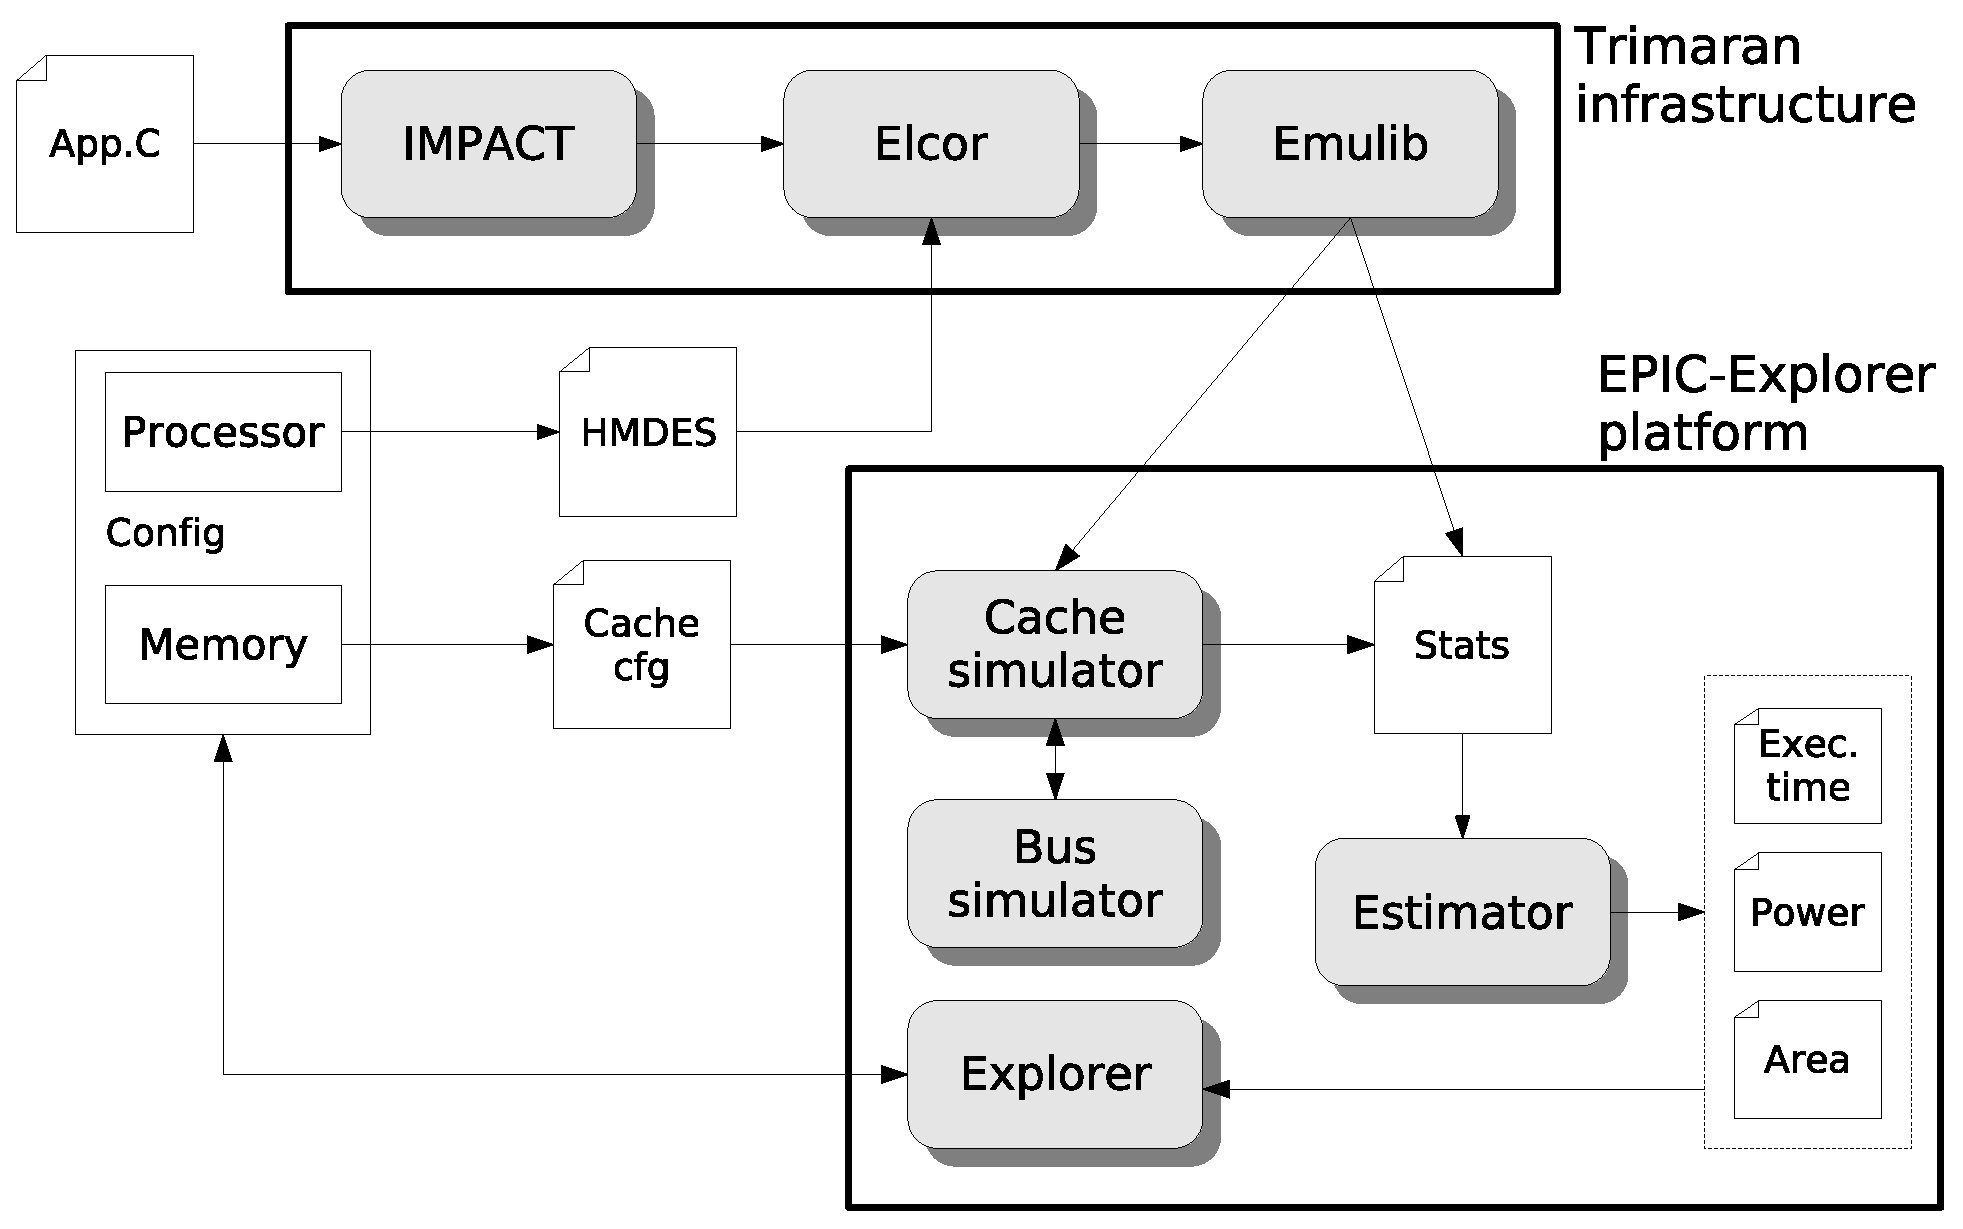
\includegraphics[width=0.65\textwidth]{pictures/evaluation_flow.eps}
        \caption{Block diagram of the framework.}
        \label{fig:evaluation_flow}
\end{figure}

The application (App.c) is first compiled by the Trimaran's compiler
front-end (IMPACT). At the end of the compilation flow,
Trimaran supplies a simulation library (Emulib) which makes it
possible to execute the VLIW code produced by Elcor, generating a file
(Stats) containing the execution statistics (e.g., instruction mix,
execution cycles, utilization of functional units, etc.). A cache
simulator, along with a bus simulator, is used to gather information
about the behavior of the memory hierarchy in terms of miss rate and
data/address traffic on the interconnection buses.

Together with the configuration of the system, the statistics produced
by simulation contain all the information needed to apply the area,
performance and power consumption estimation model implemented in the
\emph{Estimator} component. These are high-level abstraction models
that allow to quickly get an estimation while still providing a
discrete level of accuracy (for a detailed description of the models
see also~\cite{Ascia2005940}).

Finally, the results obtained by these
models are the input for the \emph{Explorer} component. This component
executes an optimization algorithm, the aim of which is to modify the
parameters of the configuration so as to minimize the three cost
functions (area, execution time and energy/power consumption).

%\subsection{Estimation Models}
%
%The average power consumed by the processor was estimated using an
%adaptation of the Cai-Lim model~\cite{cai_micro99} to the VLIW
%processor. As regards the cache subsystem, a transition-based model
%was used, according to the equations described
%in~\cite{kamble_islped97}.  The main memory energy is based on the
%model in~\cite{shiue_dac99} and assumes a per main memory access
%energy of $4.95 \times 10^{-9} J$ based on the data for the Cypress
%CY7C1326-133 memory chip.  The contribution towards power consumption
%made by the interconnection system was calculated by counting the
%number of transitions on the bus lines and applying the formula
%$P_{bus} = 1/2 V_{dd}^2 \alpha f C_l$ where $V_{dd}$ is the supply
%voltage, $\alpha$ is the switching activity, $f$ is the clock
%frequency and $C_l$ is the capacity of a bus line. For the on-chip
%buses we also considered the coupling capacitances between bus lines,
%using the model in~\cite{lekatsas_dac01}. 

\subsection{Comparison Setup}
\secL{comparison}

The results presented in the next section compare PS with one widely
adopted Multi-objective Genetic Algorithm~\cite{knowles_techrep06}. To
the best of our knowledge, genetic approaches in general still
represent the best compromise between efficiency (i.e. time required
for exploration) and accuracy of the reported Pareto Sets.  Note that,
for the reasons described above, mono-objective approaches have been
explicitly excluded from this analysis.  We also exclude other
approaches (e.g.  dependency based~\cite{givargis_tvlsi02}) that make
use of some a-priori knowledge about the role and the semantics of each
parameter, since our aim is evaluate the capacity of focusing on
interesting parameter regions without any external judgment or help
based on heuristics.  In this work, when referring to
genetic approach (or GA), we consider the widely spread 
\emph{SPEA2}~\cite{zitzler_eurogen01} variant of the Multi-objective
Genetic Algorithm, remanding to
works like~\cite{zitzler_ec00}~\cite{zitzler_tec03} for a detailed
analysis on how it could differ from other genetic approaches and what
could be expected from similar multi-objective strategies. 

Although an analogy between the concepts of ``era'' and ``generation''
can be considered, comparisons have been carried out using as
reference a fixed amount of total unique simulations, instead of a given
number of eras/generations . The purpose is to make the comparison
fair and accurate from the algorithm performance perspective, since a fixed budget of
different simulations is more directly related to the actual amount of time
required to execute the exploration.
%; on the other side, simply
%referring to a given number of generations/eras could be inaccurate
%when a considerable number of configurations remain unaltered in the
%current population (e.g. because of a local optimum)

The set of default algorithm tuning parameters used for both the
genetic and PS approaches is shown in
Table~\ref{tab:defaults}. Given the similarity, both in terms of
meaning and functionality, between the parameter $K$ and the population size
of the genetic approach, they both have been set to the same values. As discussed
when introducing the main PS algorithm concepts, a sensitivity analysis on the algorithm parameters is beyond the scope of this work. Nevertheless, we conducted several tests with
different values of $K$, similar to the ones shown in
Figure~\ref{fig:kimpact}, which refers to the alloca\_test application
and a total budget of 500 configurations. We found that initially increasing values
of $K$ seems to improve both Pareto front (as in the picture on the left) and objective
distribution (on the right), but, after some threshold value, $K$ does
not seem to provide any benefit, even returning to slightly worse
results for the last values of $K$ considered (100). Similar trends have been
found for the other benchmarks (not included for space reasons),
showing on average a value of $K$ around 30 as
reasonable sweet spot for the objectives. A complete resource with the
whole set of results and data obtained in the tests performed can be found online
at~\cite{ps_results}.

\begin{table}
	\tbl{Algorithm Parameters\label{tab:defaults}}{
	\begin{tabular}{cll}
	\hline
	\multicolumn{1}{c}{Algorithm} & \multicolumn{1}{c}{Parameter} & \multicolumn{1}{c}{Default Value} \\
	\hline
	GA & population size & 30 \\
	GA & crossover probability & 0.8 \\
	GA & mutation probability  & 0.1 \\
	PS & era budget ($K$) & 30 \\
	PS & innovation threshold ($\alpha$ ) & 1 \\
	both PS and GA & Total simulations budget & 100-500 \\
	\hline
	\end{tabular}}
\end{table}

\begin{figure}
  \figLC{kimpact}{Impact of increased K values on Pareto fronts and distribution for the alloca\_test application. }
  \begin{center}
    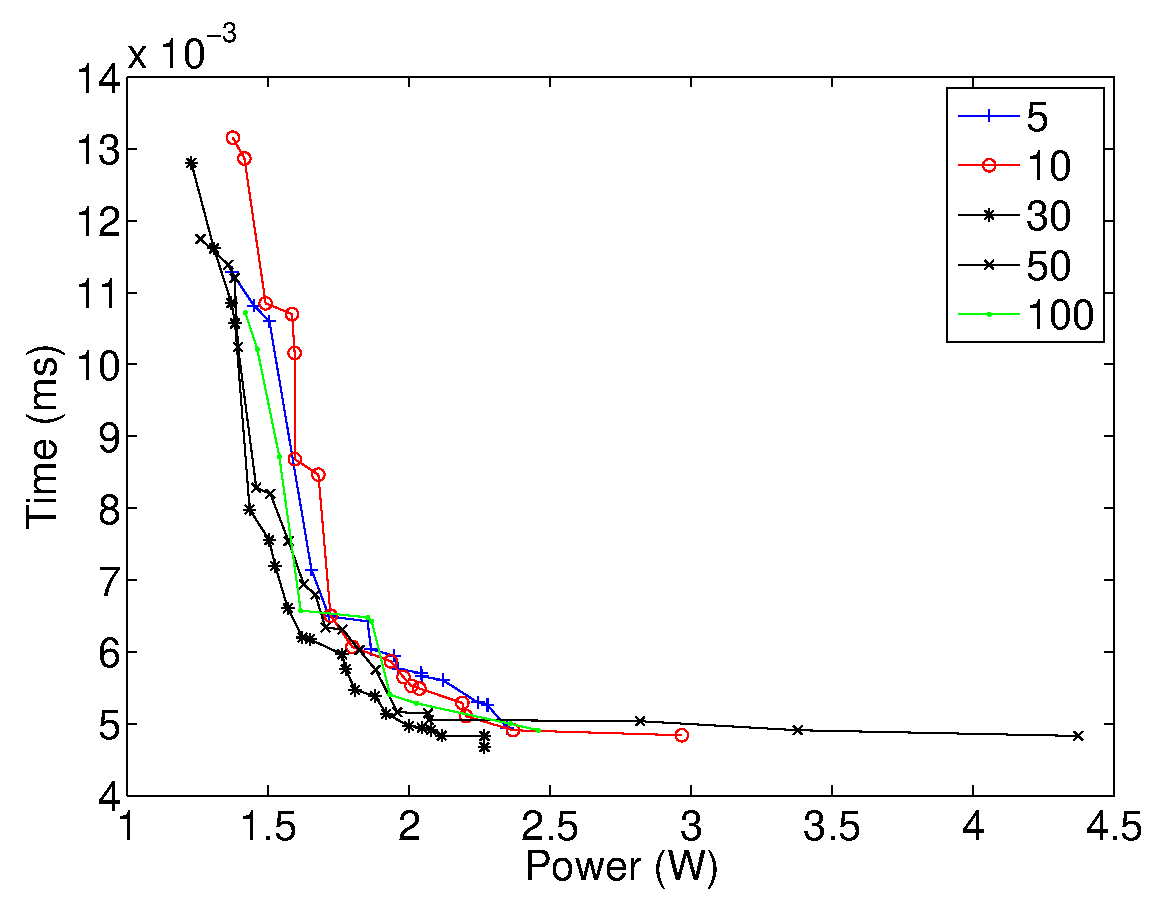
\includegraphics[width=0.45\textwidth]{pictures/alloca_K.eps} 
    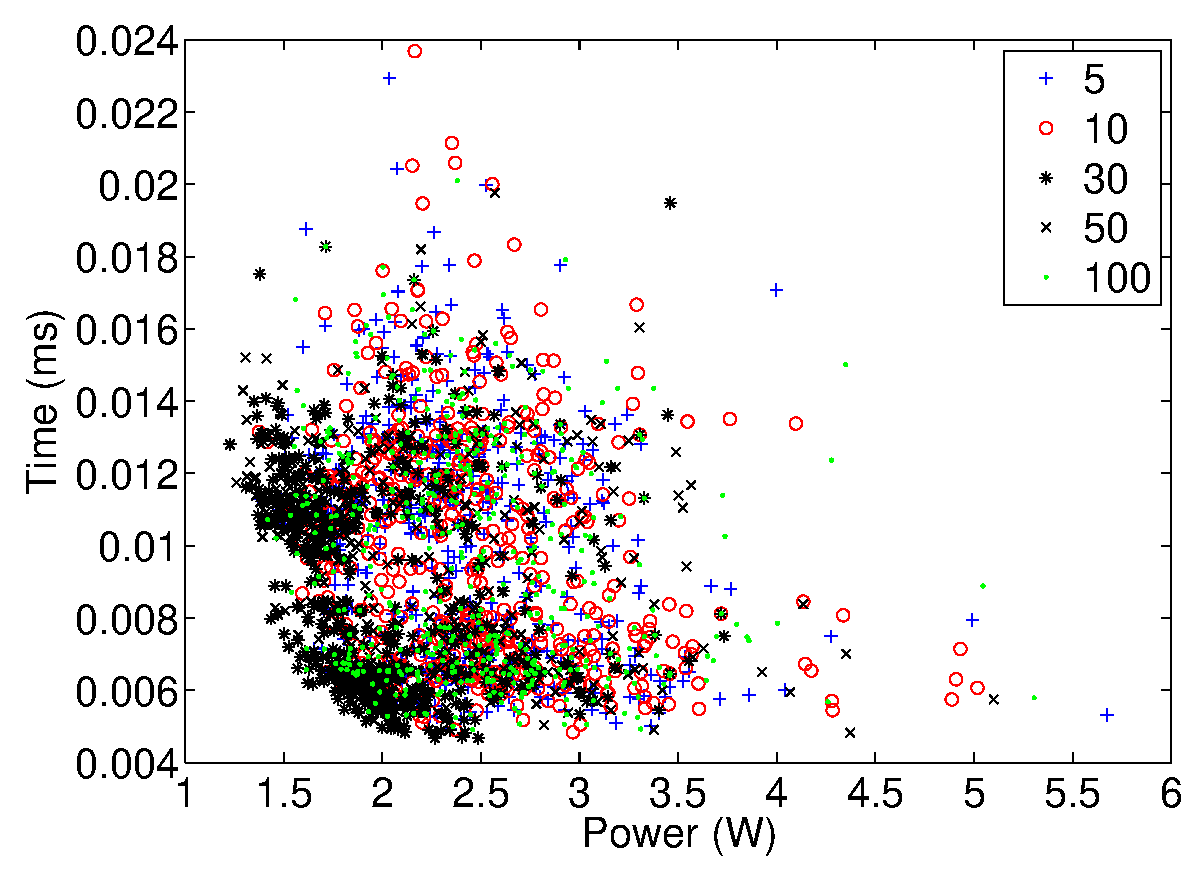
\includegraphics[width=0.45\textwidth]{pictures/alloca_K_ALL.eps} 
  \end{center}
\end{figure}

%------------------------------------------------------------------------------

\subsection{Evaluation metrics}
\secL{metrics}
A qualitative evaluation of Paretos is probably the simplest way to
have a quick glance on algorithm behavior and results. However, in
tests involving a comparison between different exploration strategies,
this approach could not help in capturing the whole picture, missing
some important properties related to the distribution of the solutions
found.
In order to evaluate the Paretos from a quantitative point-of-view we
will consider two metrics, namely, the \emph{variation range} and the
\emph{average normalized absolute dispersion error}. Both of them permit to quantify the extent of the Pareto front that is an important factor to consider when evaluating its quality. Indeed, authors of \cite{zitzler_ec00,weise2012evolutionary} observe that an exploration algorithm should preferably provide Pareto fronts whose objective function range is large. In other words, following the terminology of~\cite{weise2012evolutionary}, a \emph{uniform convergence} should be guaranteed.
Pareto fronts with large objective function ranges permit to investigate in a broader way the potentials of the designed device. This is important, in general, since if only a narrow portion of the Pareto front is provided due to non-uniform convergence, the decision maker may neglect some important options~\cite{weise2012evolutionary}. Having a wide Pareto front becomes essential, in particular, when designing a device that may be required to satisfy different constraints. For example, the decision maker may want to design two different multi-purpose processors. The first design may adapt to situations in which the processor is used for real time elaboration (thus requiring low execution time) and is attached to the powerline (thus not having stringent power dissipation constraints). The second design, on the contrary, may fit situations in which the energy is provided by a battery (stringent power constraints) but only background computations are performed (long execution time is tolerable). These two processors may be successfully designed maintaining the same architecture and simply using different values for the design parameters. A wide Pareto front helps in achieving this goal.

For a given objective, the \emph{variation range} represents the ratio
between the maximum and the minimum value observed for that objective.

Another metric is the average \emph{normalized absolute dispersion
error}: it measures
the average absolute difference between the distribution of points in
the objective space and an ideal distribution in which the points are
uniformly distributed over the objective space. 
Formally, let $O$ be
the image, in the objective space, of the configurations visited by
the design space exploration. The generic element of $O$ (\ie, a
solution) is a pair $(p,t)$ where $p$ and $t$ are the average power
and execution time, respectively. The two-dimensional objective space
is then partitioned by a $M_x \times M_y$ mesh. For each tile $T_i,
\ i=1, 2, \ldots, M_xM_y$ of the mesh, let $N_i$ be the number
of points in $O$ which fall in $T_i$. The average absolute error, $E_i$, for
$T_i$ is the absolute value of the difference between $N_i$ and the
ideal number of solutions, $\overline{N}$, which should fall in $T_i$
in case of uniform distribution. Such $\overline{N}$ can be simply
computed as the ratio between the cardinality of $O$ and the number of
tiles. Thus,
\[ E_i = |N_i - \overline{N}|, \]
where $\overline{N} = |O| / (M_x M_y)$. The average
normalized absolute dispersion error ($ANADE$) is the average of $E_i$
normalized to the maximum absolute error $E_{max}$:
\[ ANADE = \frac{\sum_{i=1}^{M_xM_y} E_i/(M_xM_y)}{E_{max}}, \]
where $E_{max}$ can be computed as the average absolute error in the worst
case in which all the solutions fall in a single tile:
\[ E_{max} = \frac{(M_x M_y - 1) \overline{N} + |\overline{N} -
    |O|| }{M_x M_y}. \] 

%\subsection{Impact of the algorithm parameters}
%\secL{parameter_impact}
%\comment{IMPACT OF $K$. Si potrebbero presentare un plot in cui il numero totale di simulazioni e' fissato e vengono eseguiti diversi run dell'algoritmo con diversi valori di K. Per ogni run, il pareto set e' rappresentato nel plot, sottoforma di una curva diversa. Mi aspetterei che tutte le curve siano molto simili. Per ciascun run, il valore di variation range e average absolute dispersion error sono riportati. Mi aspetto valori simili, il che confermerebbe che la diversity nel nostro algoritmo non dipende da $K$. Ne vale la pena rifare questi run? Ci vuole troppo tempo?} 
%
%\comment{Si potrebbe mettere un plot con nelle ascisse l'era e nelle ordinate il numero di split avvenuti in quell'era. Si potrebbero disegnare diverse curve, una per ogni valore di alpha, per far vedere che il numero di split e' piu' alto q. Recommended values are close to 1, as results in \secR{ee} confirm. Using different values, if sufficiently close to 1, does not have a considerable impact on the resulting Pareto front approximation. Ne vale la pena rifare questi run? Ci vuole troppo tempo?}

\subsection{Results}

In this Section we first analyze the results of GA and PS approaches from a
qualitative perspective, showing how Pareto curves compare when
plotted on the bidimensional space of power and performance
objectives. Next, we perform a quantitative
analysis of the results in order to more accurately figure out in which
features/properties the two approaches differentiate.

\figR{pareto_fronts_100} and \figR{pareto_fronts_500} show the
resulting Pareto fronts for two scenarios of 100 and 500
simulation budget, respectively. The set of algorithm parameters involved and their
values are the ones previously shown in Table~\ref{tab:defaults}. It
should be pointed out again that the number of generations (or eras)
has been chosen so that only the given amount of different simulations is
actually performed. Thus, when accounting these simulations only
unique simulations have been considered, removing repetitions and
unfeasible configurations.

% IEEE table style
%\begin{table}
%  \centering
%  \begin{tabular}{ccc}
%    \includegraphics[width=0.30\textwidth]{pictures/alloca_100.eps} &
%    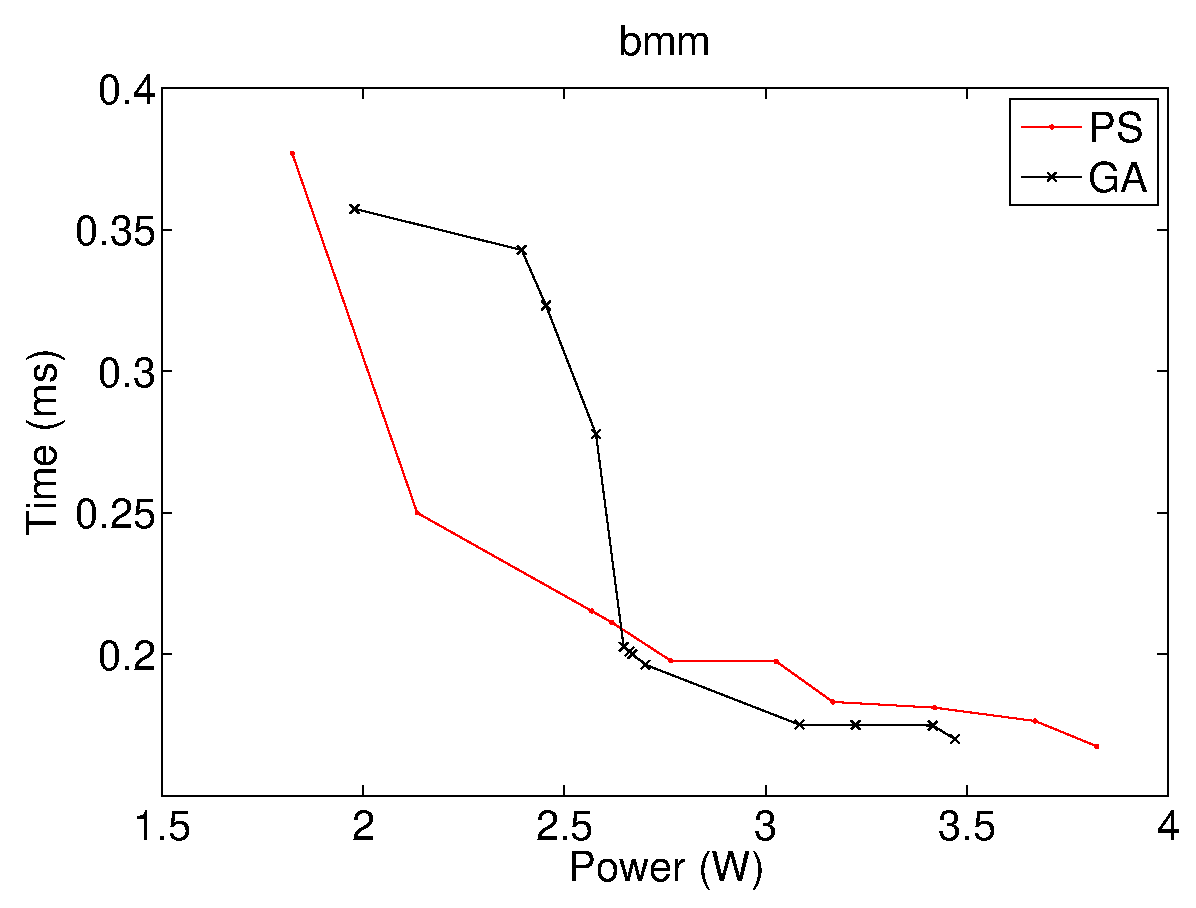
\includegraphics[width=0.30\textwidth]{pictures/bmm_100.eps} & 
%    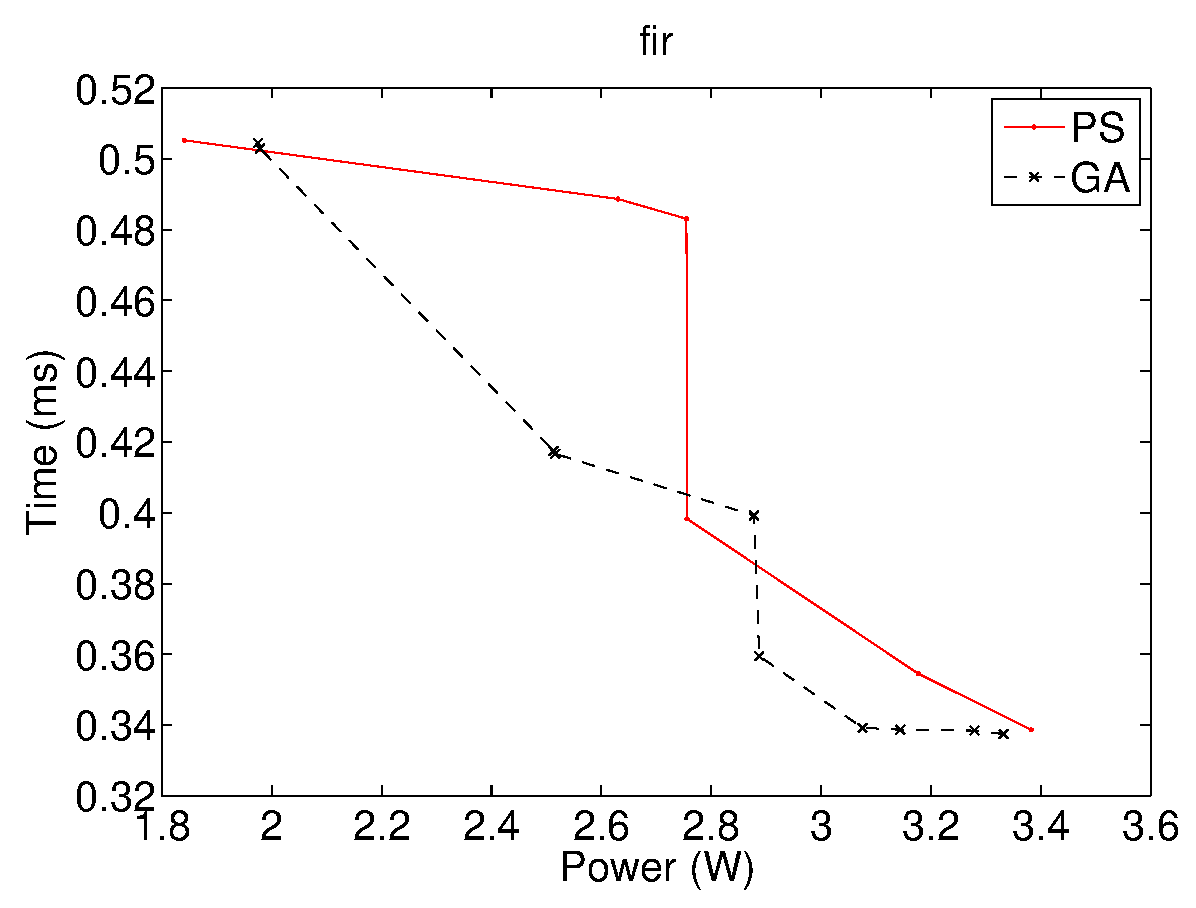
\includegraphics[width=0.30\textwidth]{pictures/fir_int100.eps} \\
%    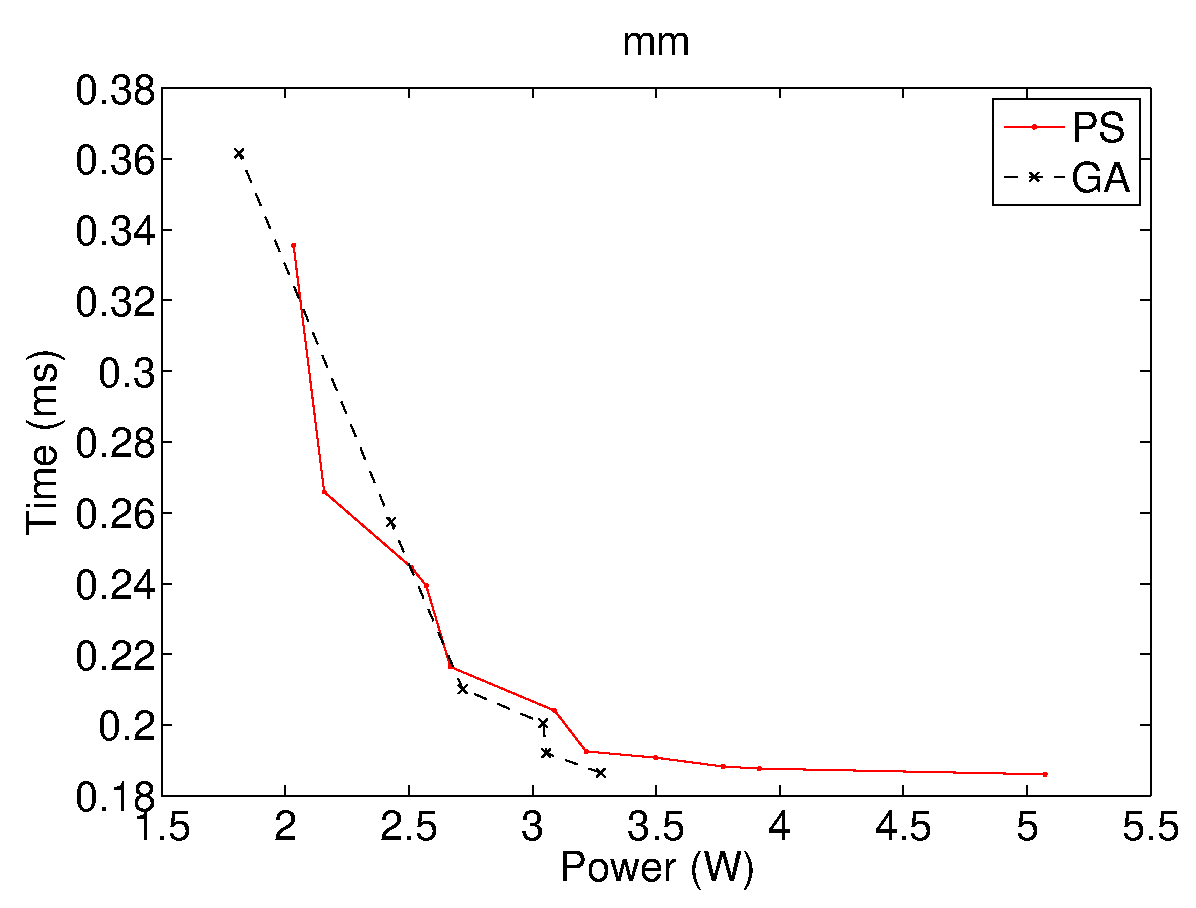
\includegraphics[width=0.30\textwidth]{pictures/mm_100.eps} &
%    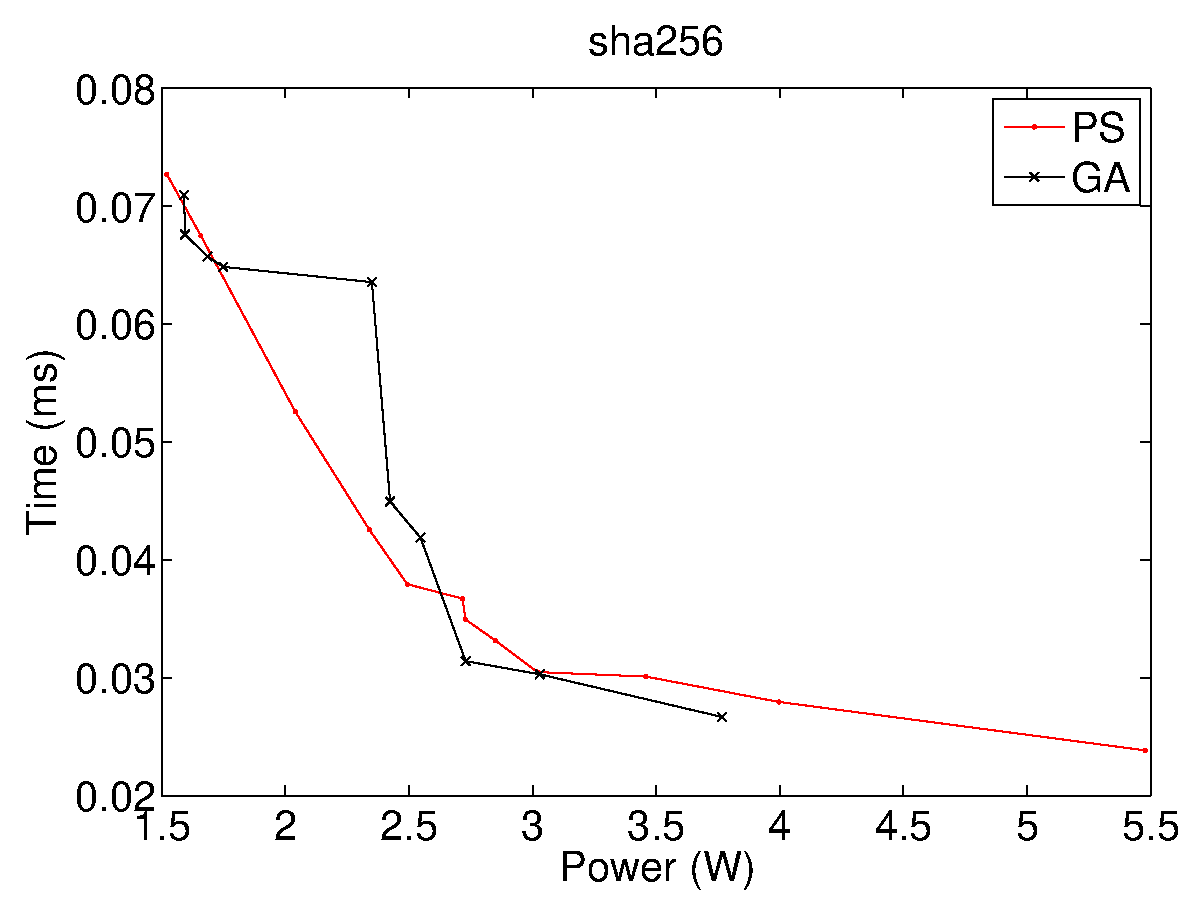
\includegraphics[width=0.30\textwidth]{pictures/sha_100.eps} &
%    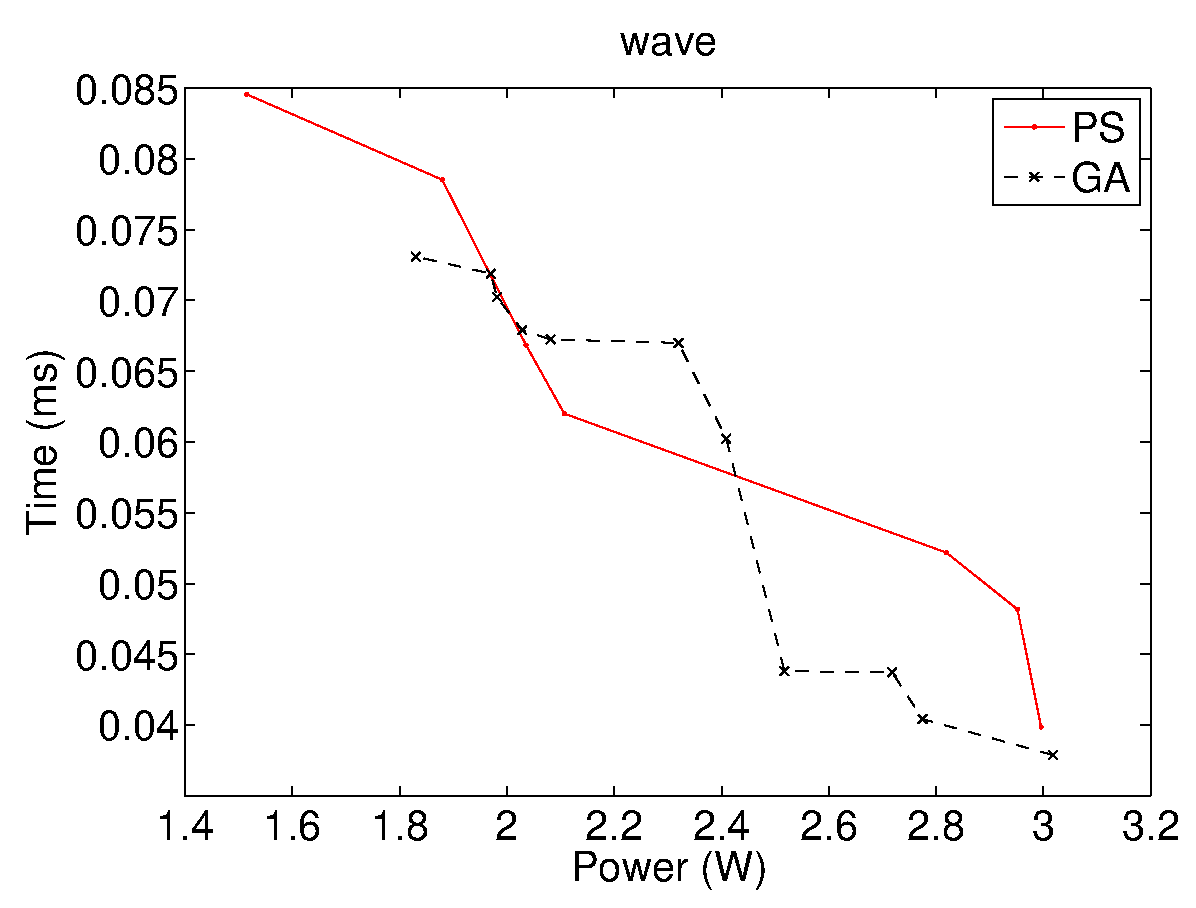
\includegraphics[width=0.30\textwidth]{pictures/wave_100.eps} 
%  \end{tabular}
%  \caption{Pareto fronts found by PS and GA for a fixed budget of 100 configurations.}
%  \label{fig:pareto_fronts_100}
%\end{table}
%
%\begin{table}
%  \centering
%  \begin{tabular}{ccc}
%    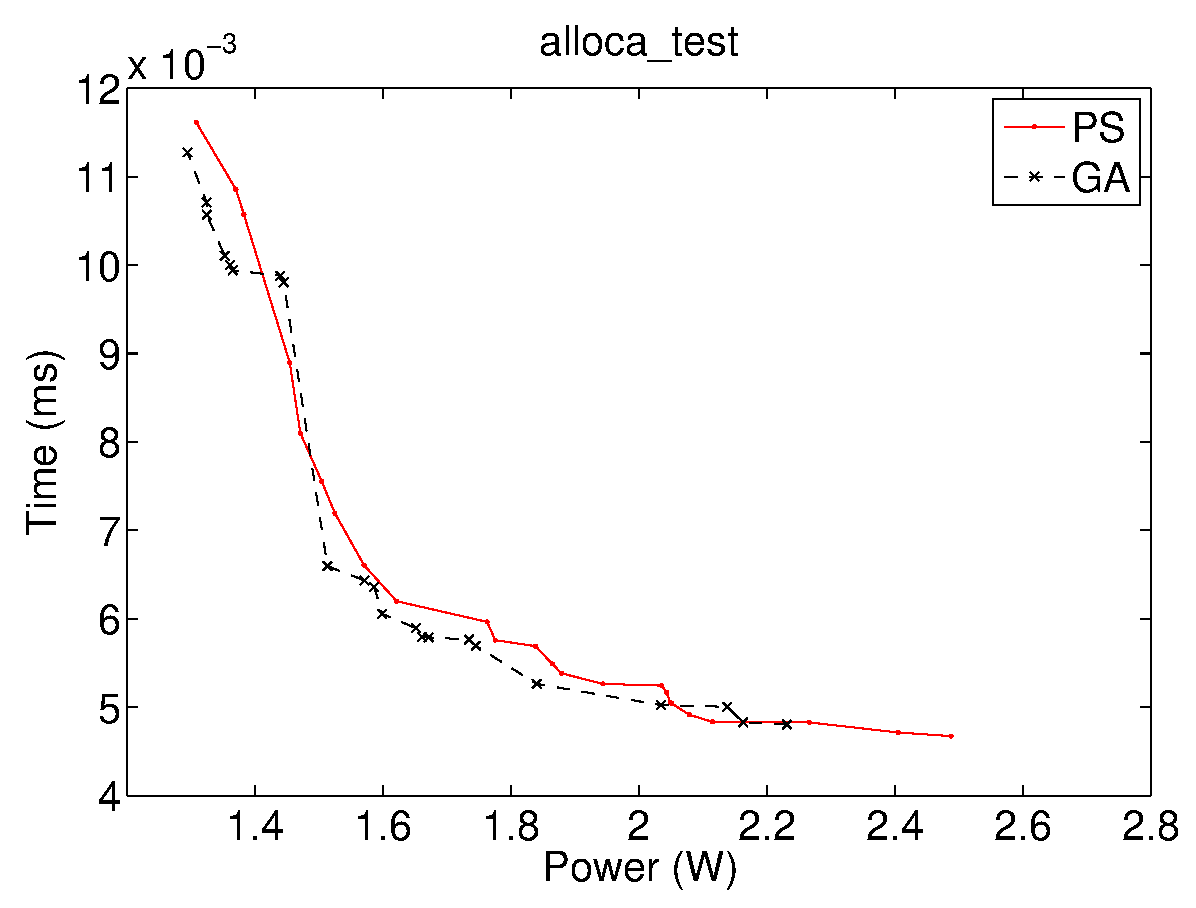
\includegraphics[width=0.30\textwidth]{pictures/alloca_500.eps} &
%    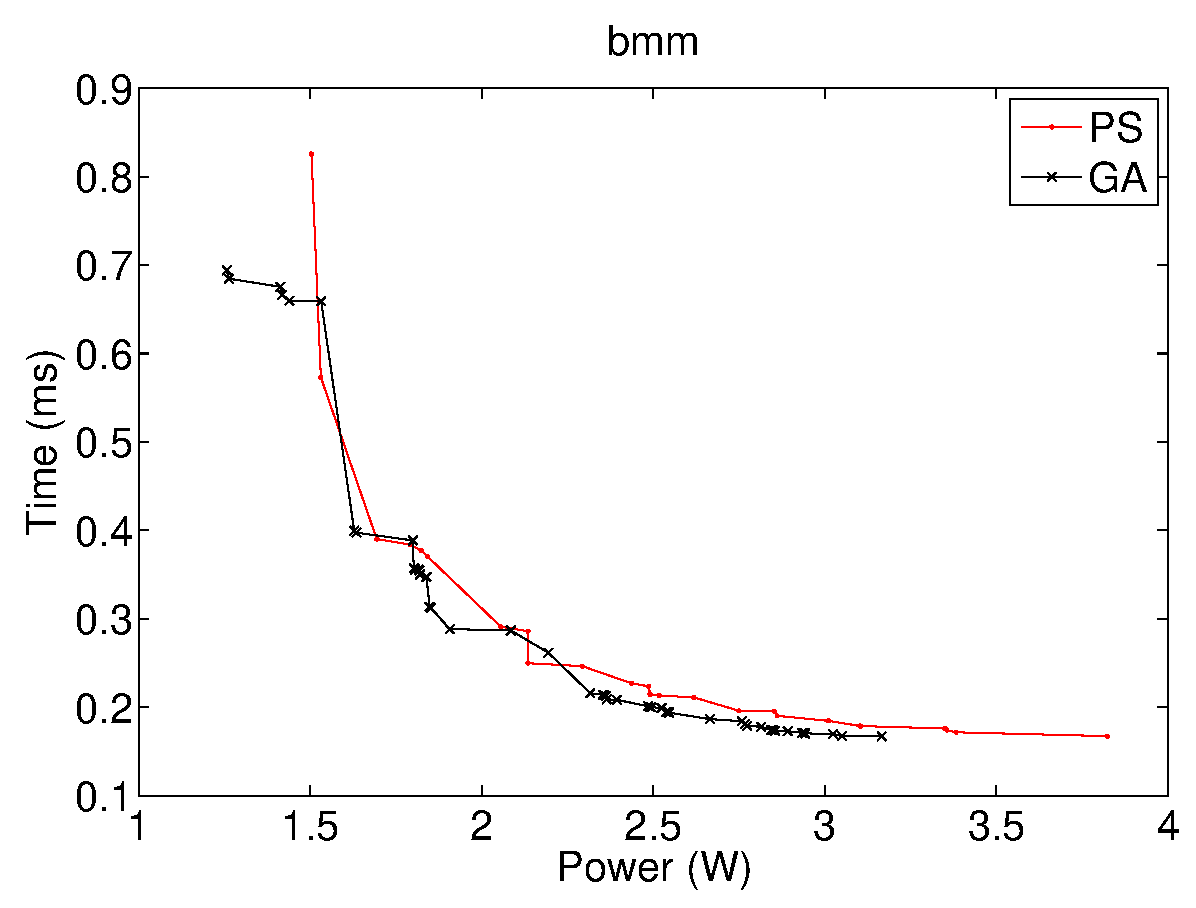
\includegraphics[width=0.30\textwidth]{pictures/bmm_500.eps} & 
%    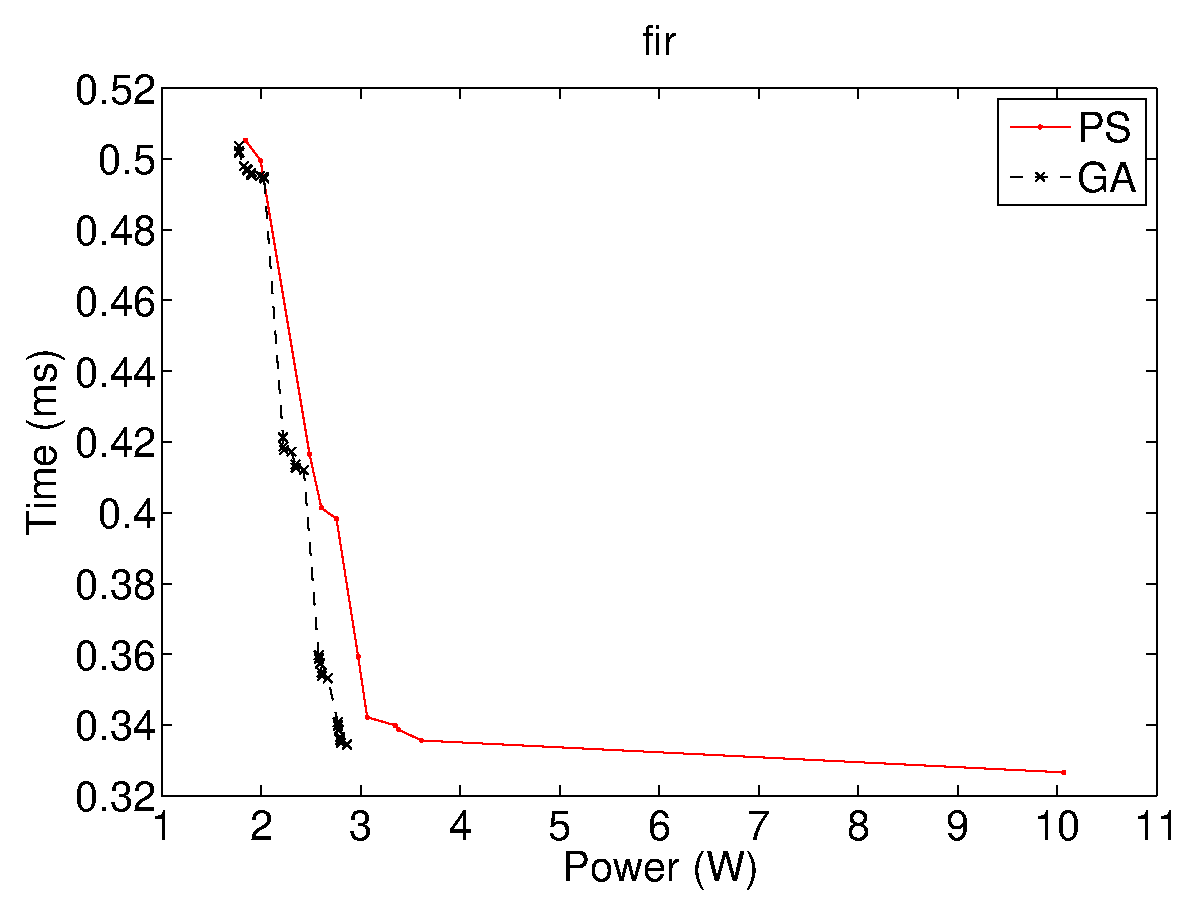
\includegraphics[width=0.30\textwidth]{pictures/fir_int500.eps} \\
%    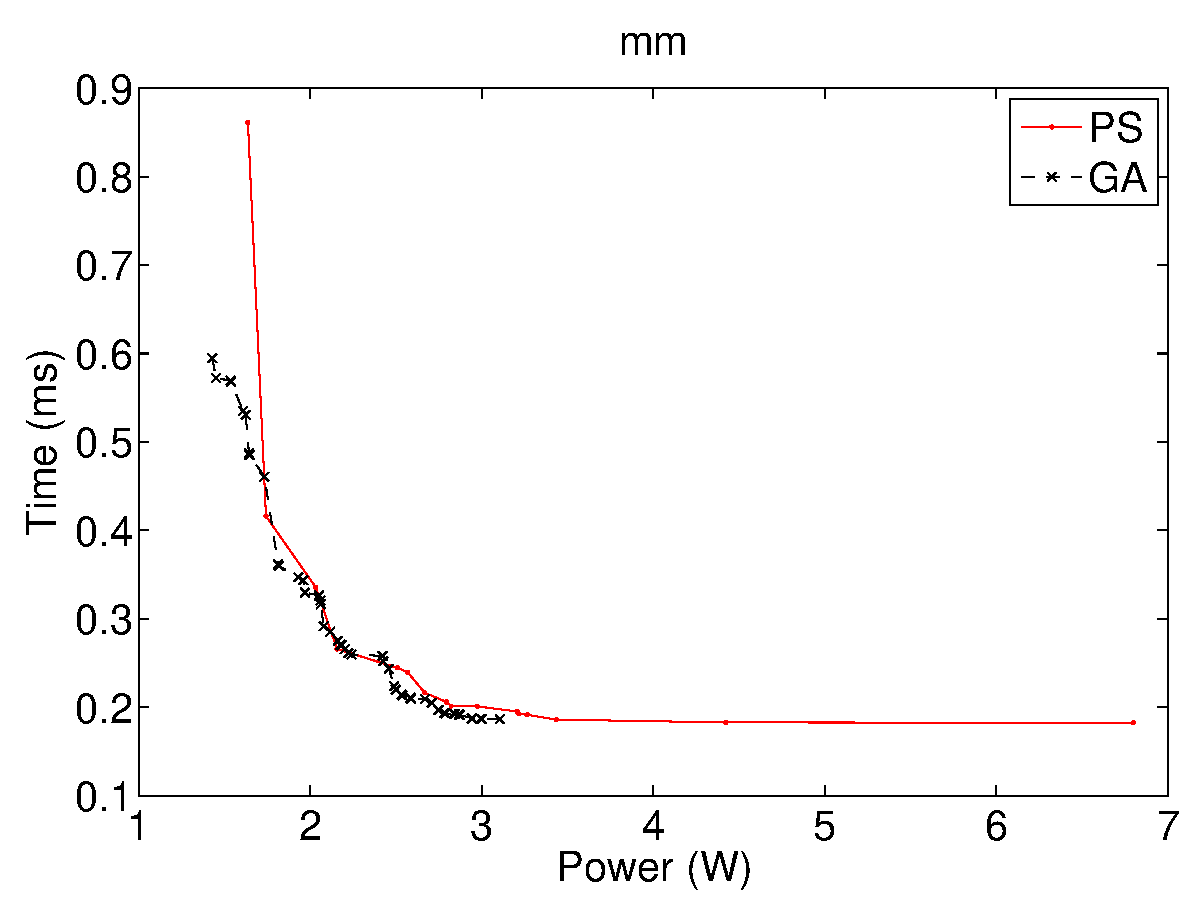
\includegraphics[width=0.30\textwidth]{pictures/mm_500.eps} &
%    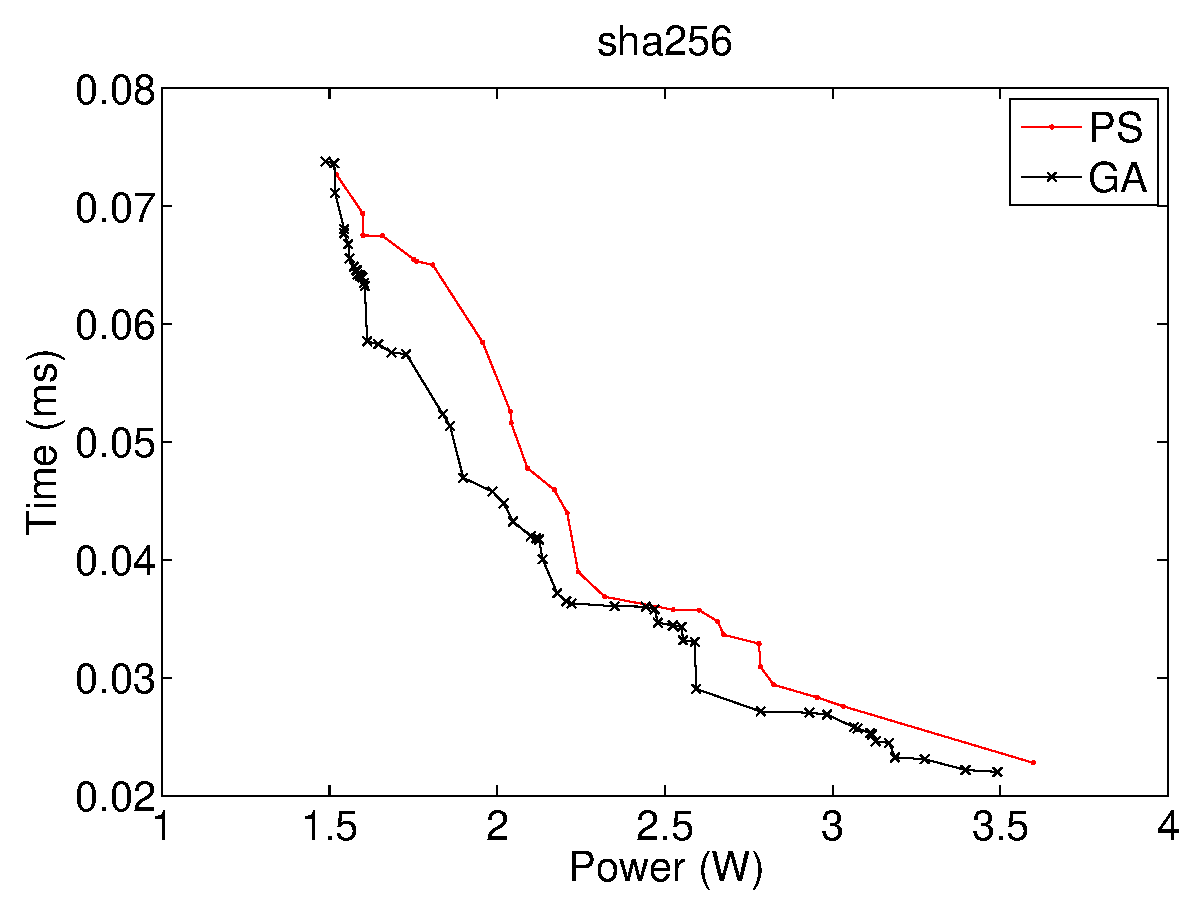
\includegraphics[width=0.30\textwidth]{pictures/sha_500.eps} &
%    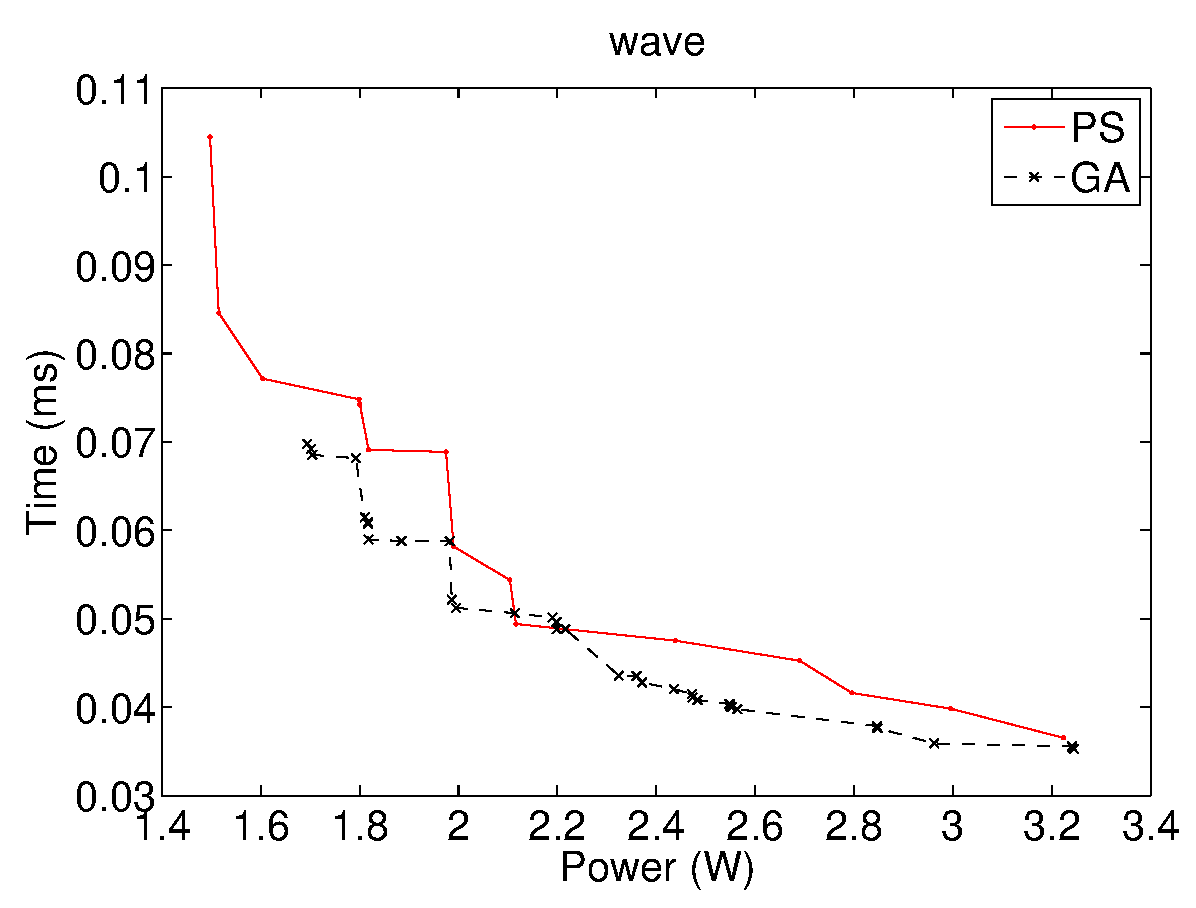
\includegraphics[width=0.30\textwidth]{pictures/wave_500.eps} 
%  \end{tabular}
%  \caption{Pareto fronts found by PS and GA for a fixed budget of 500 configurations.}
%  \label{fig:pareto_fronts_500}
%\end{table}


\begin{figure}
  \figLC{pareto_fronts_100}{Pareto fronts found by PS and GA for a
  fixed budget of 100 configurations.}
  \begin{center}
    \includegraphics[width=0.30\textwidth]{pictures/alloca_100.eps}
    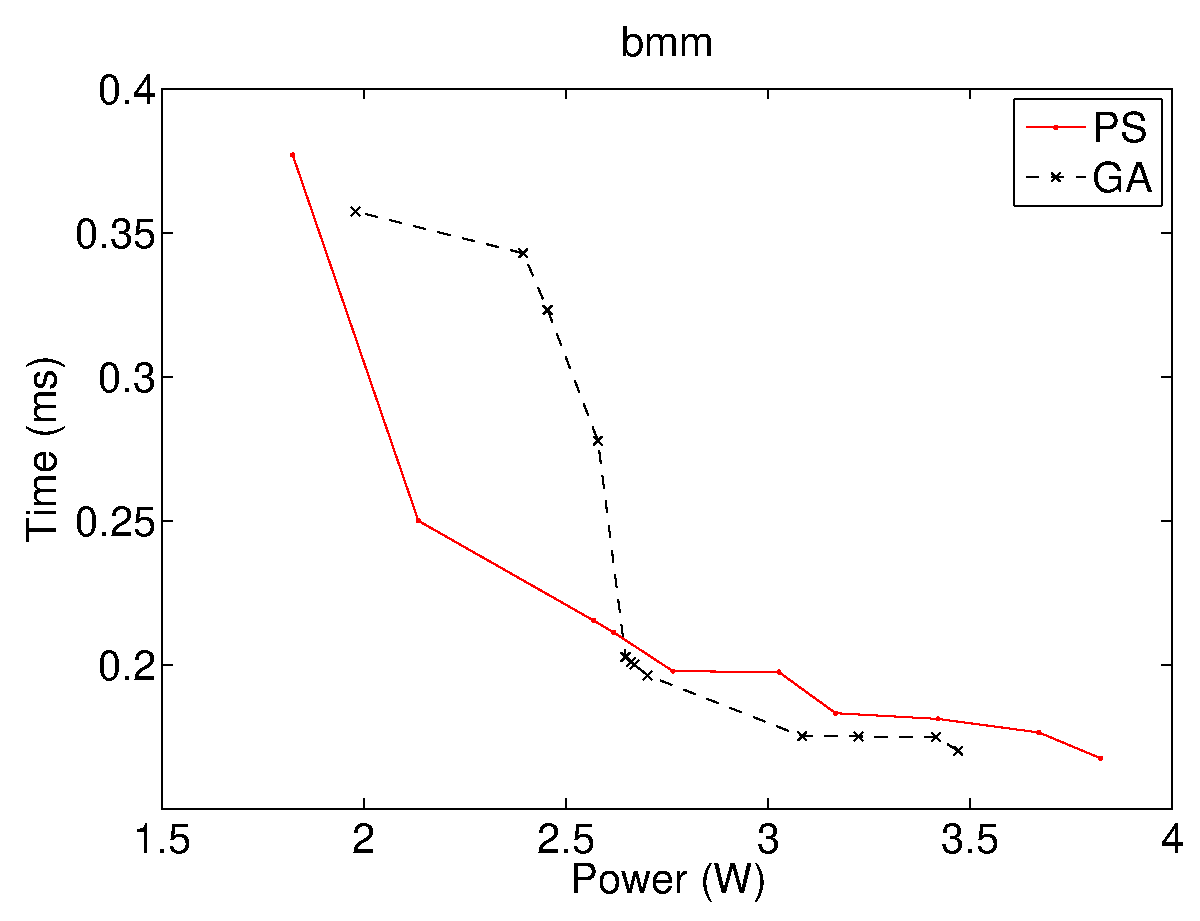
\includegraphics[width=0.30\textwidth]{pictures/bmm_100_bis.eps}
    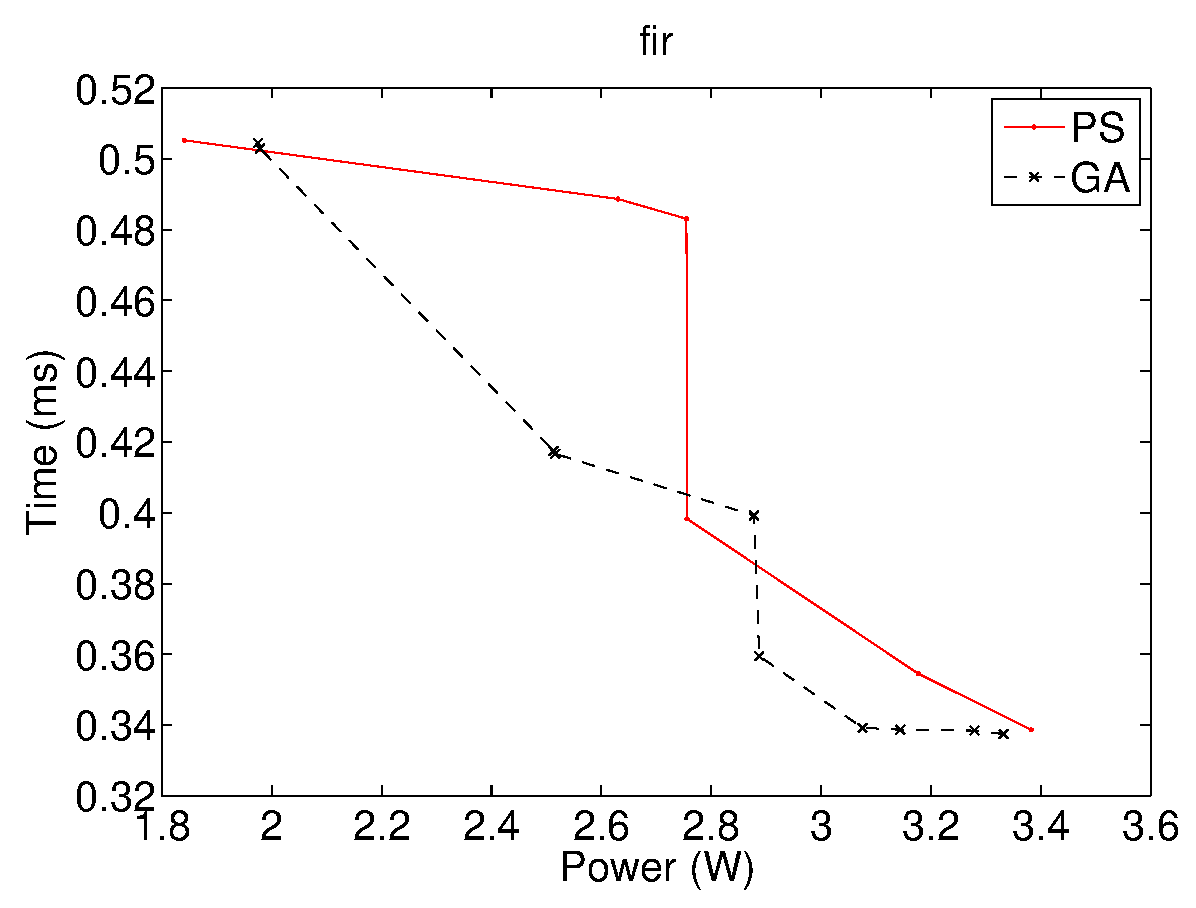
\includegraphics[width=0.30\textwidth]{pictures/fir_int100.eps}
    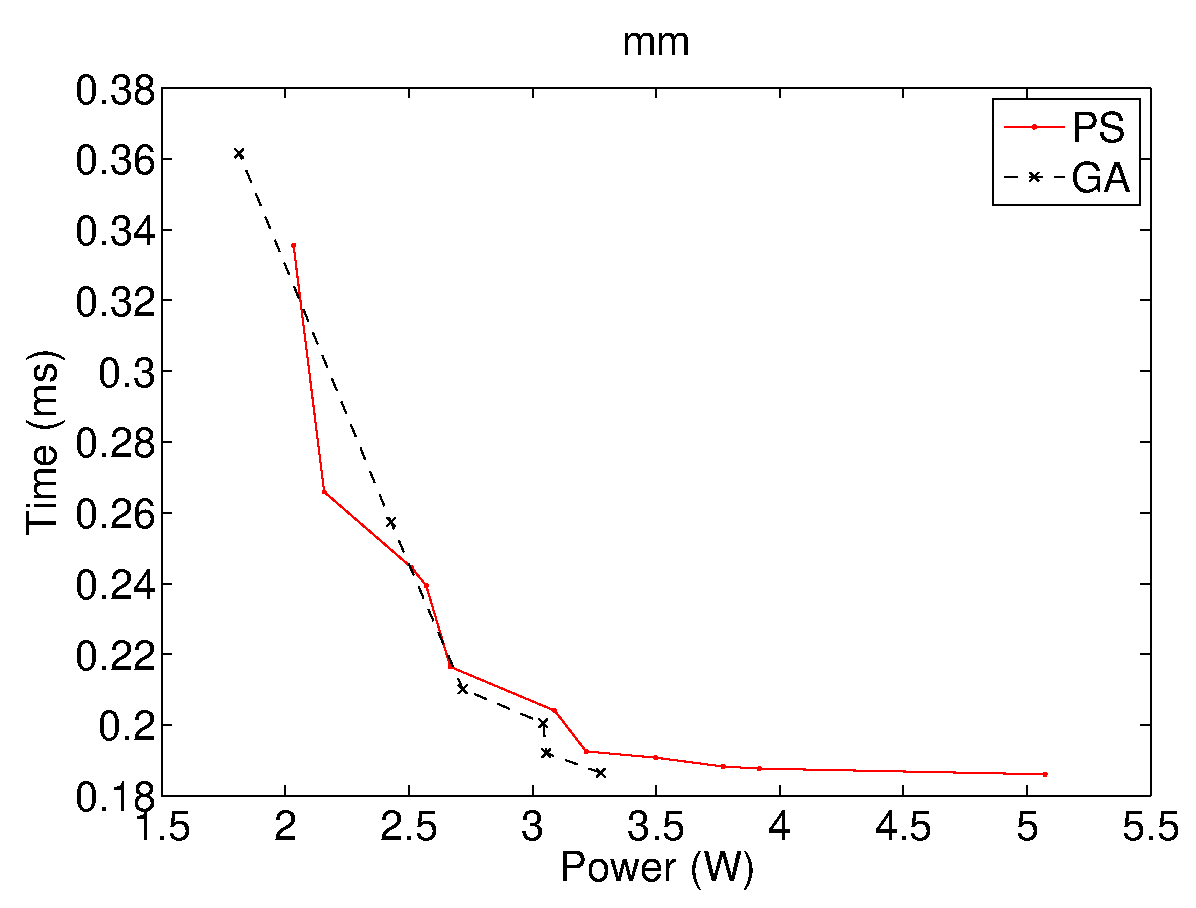
\includegraphics[width=0.30\textwidth]{pictures/mm_100.eps}
    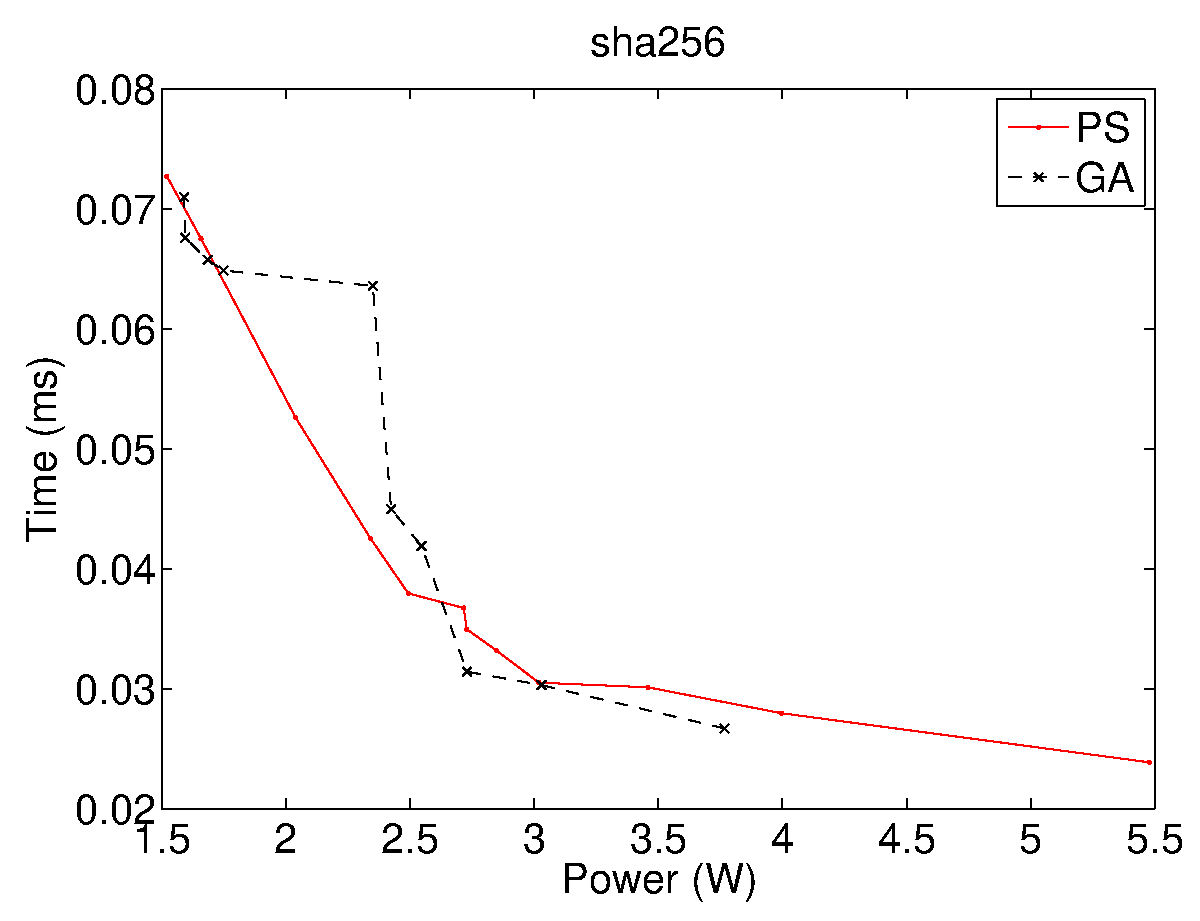
\includegraphics[width=0.30\textwidth]{pictures/sha_100_bis.eps}
    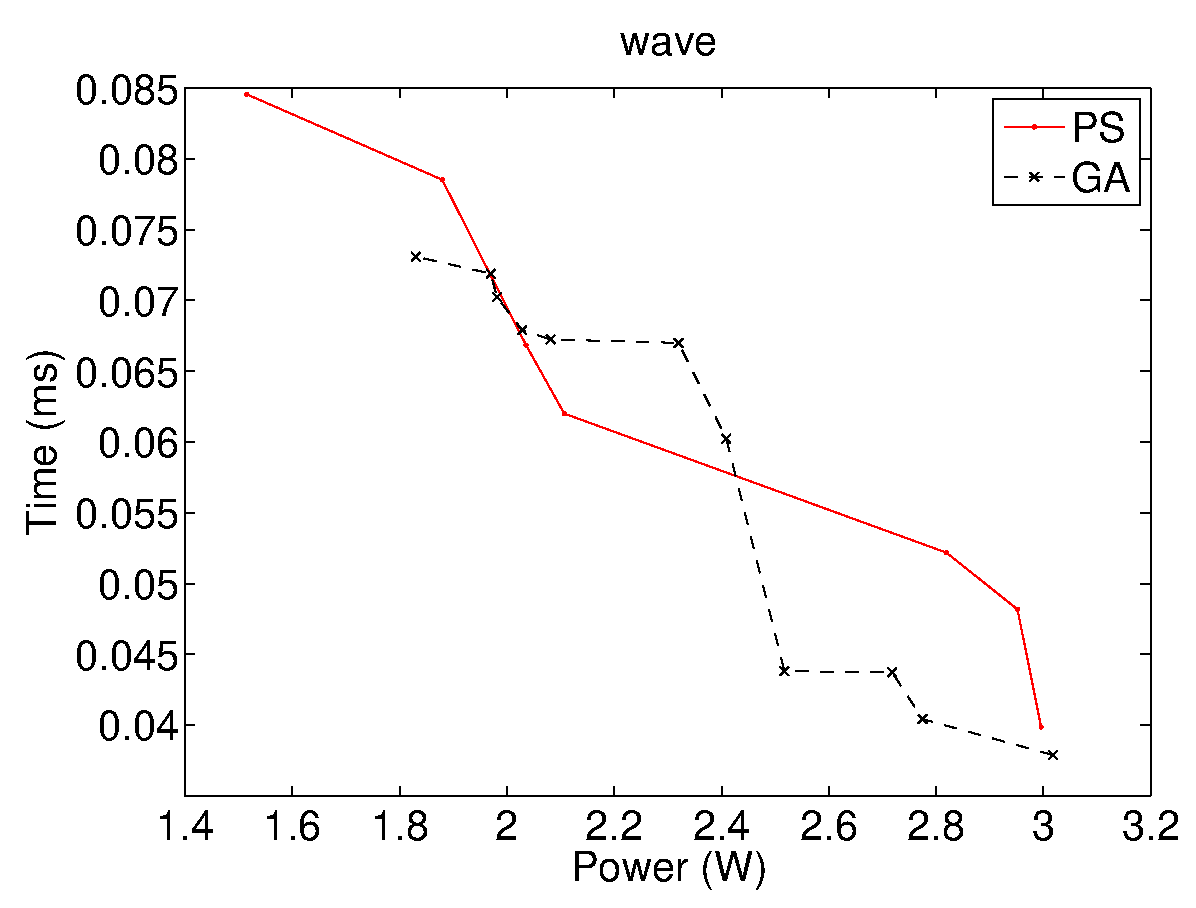
\includegraphics[width=0.30\textwidth]{pictures/wave_100.eps} 
  \end{center}
\end{figure}

\begin{figure}
  \figLC{pareto_fronts_500}{Pareto fronts found by PS and GA for a
  fixed budget of 500 configurations.}
  \begin{center}
    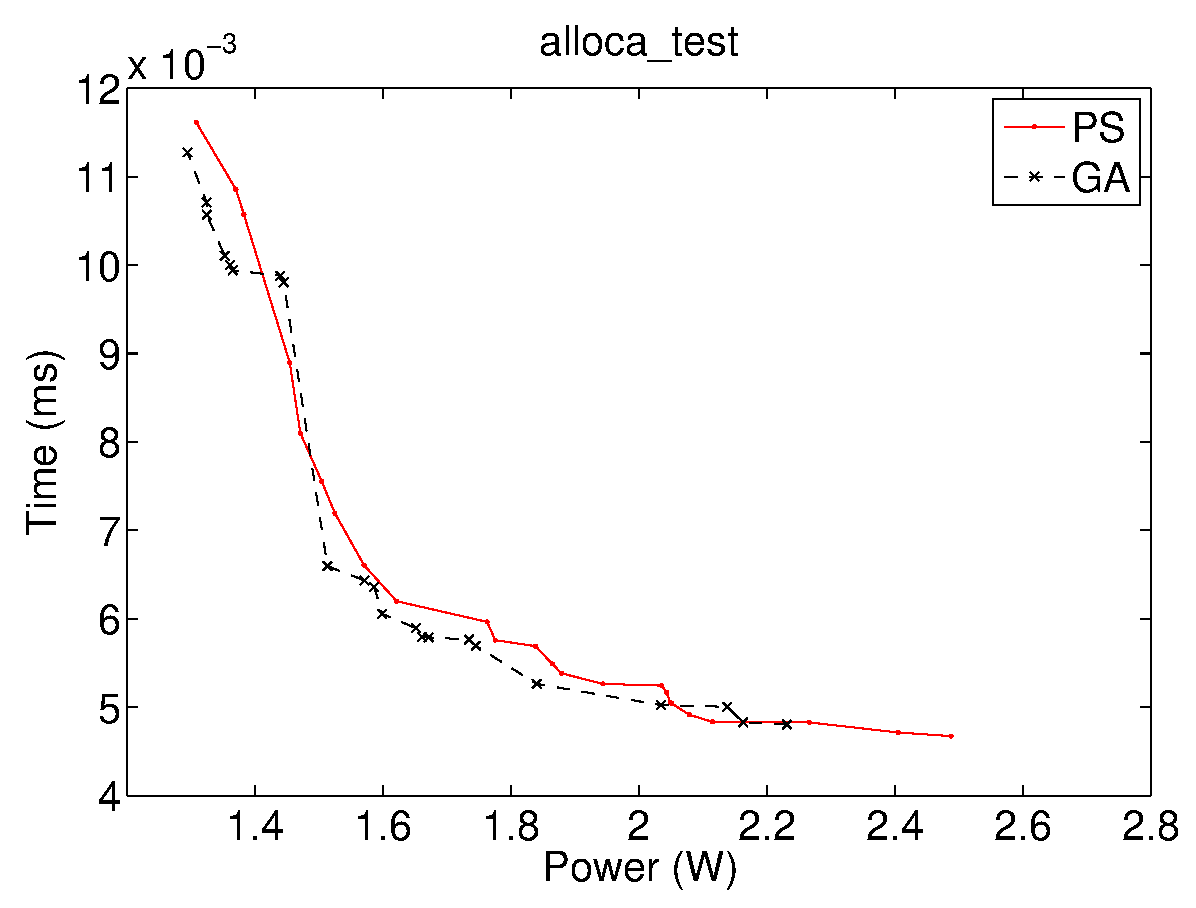
\includegraphics[width=0.30\textwidth]{pictures/alloca_500.eps}
    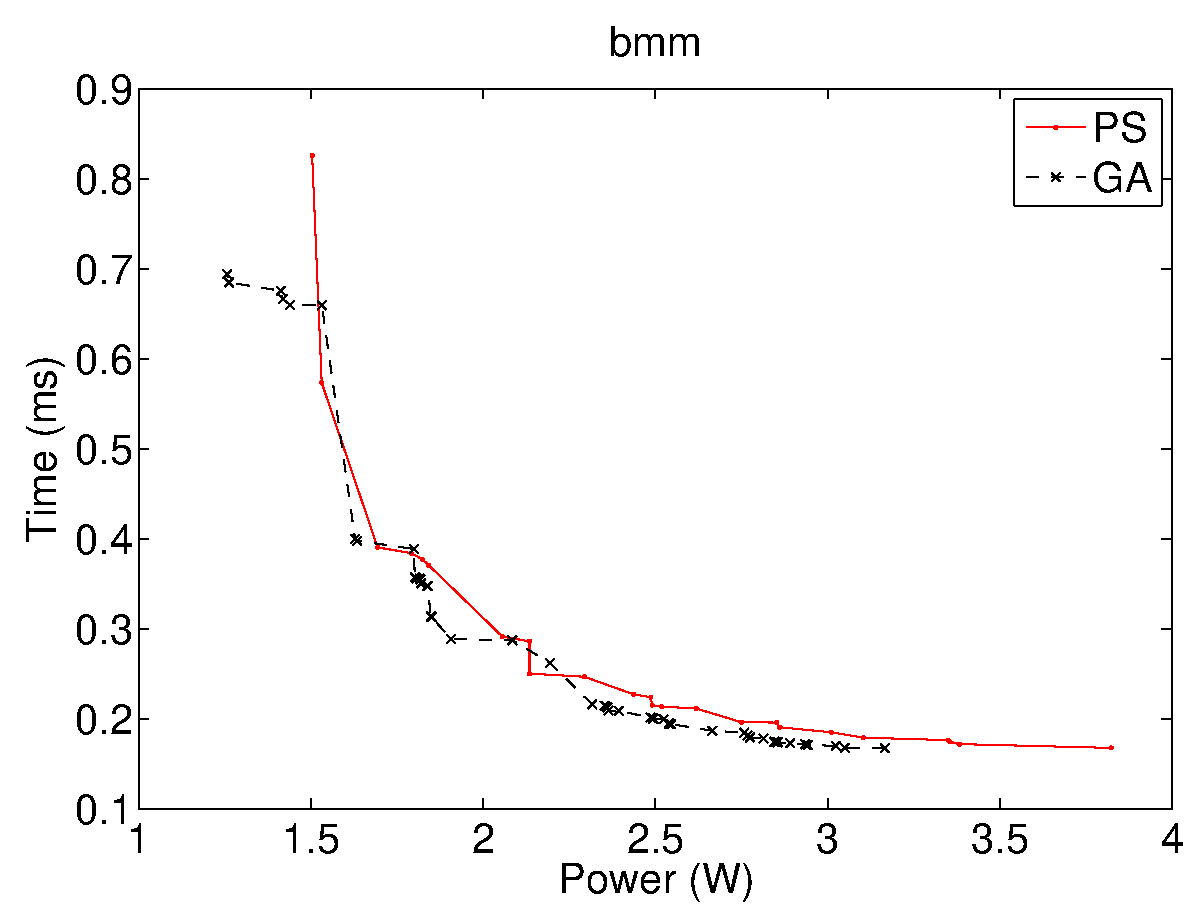
\includegraphics[width=0.30\textwidth]{pictures/bmm_500_bis.eps}
    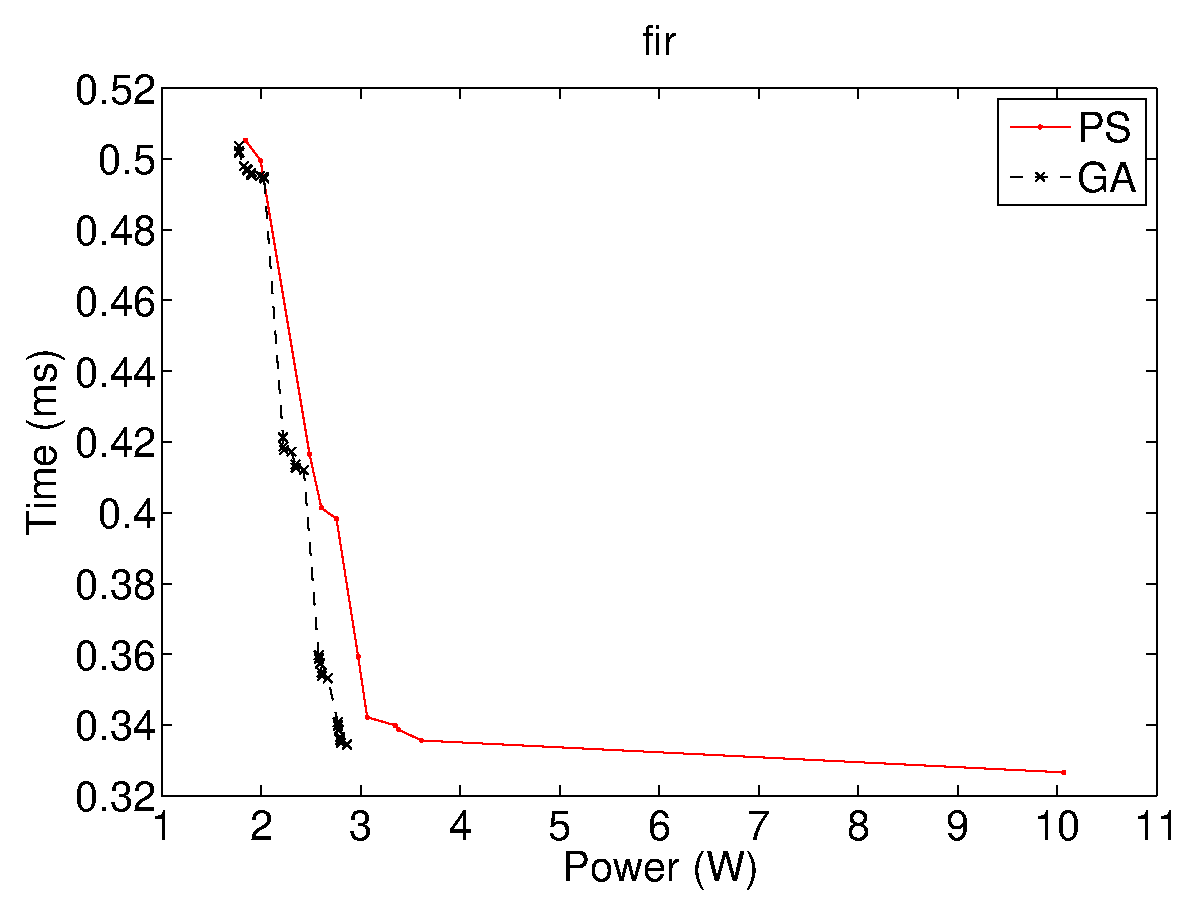
\includegraphics[width=0.30\textwidth]{pictures/fir_int500.eps}
    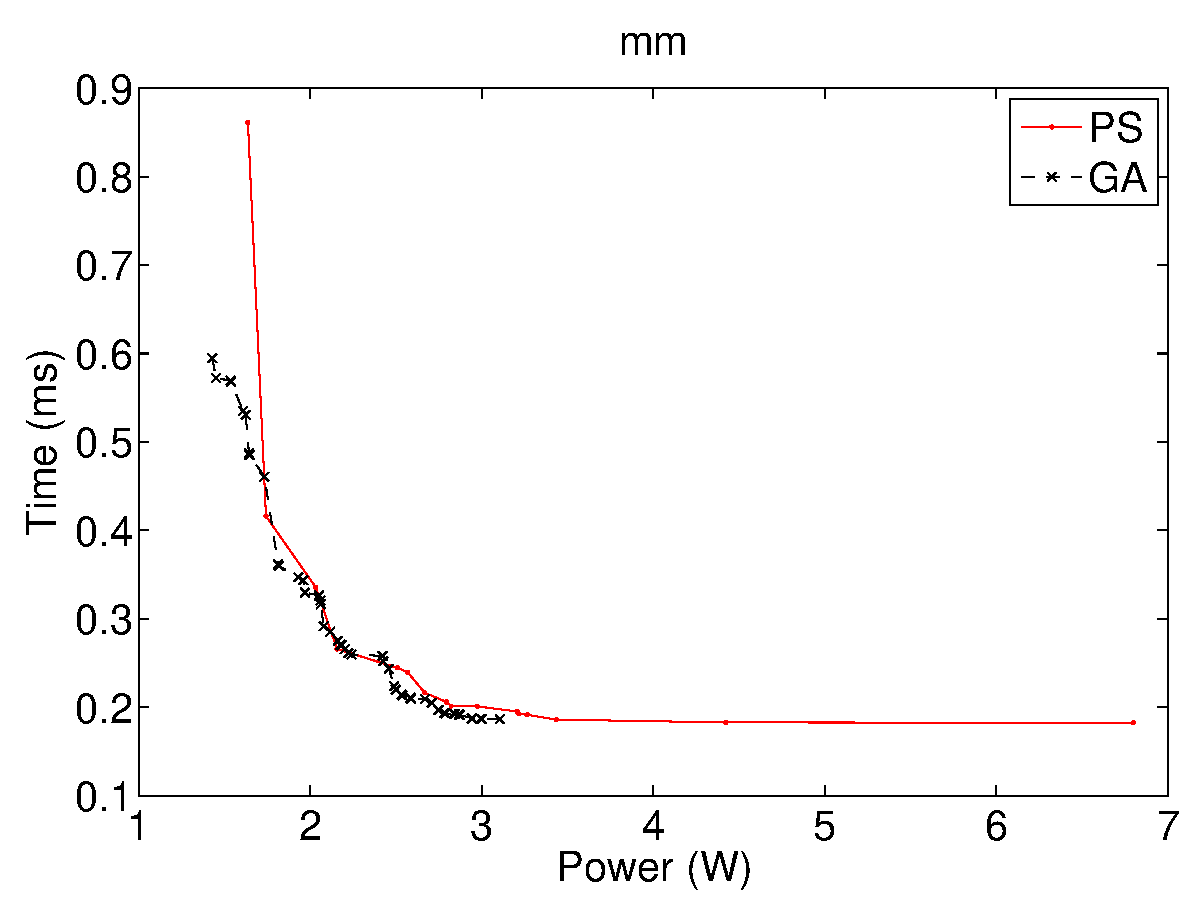
\includegraphics[width=0.30\textwidth]{pictures/mm_500.eps}
    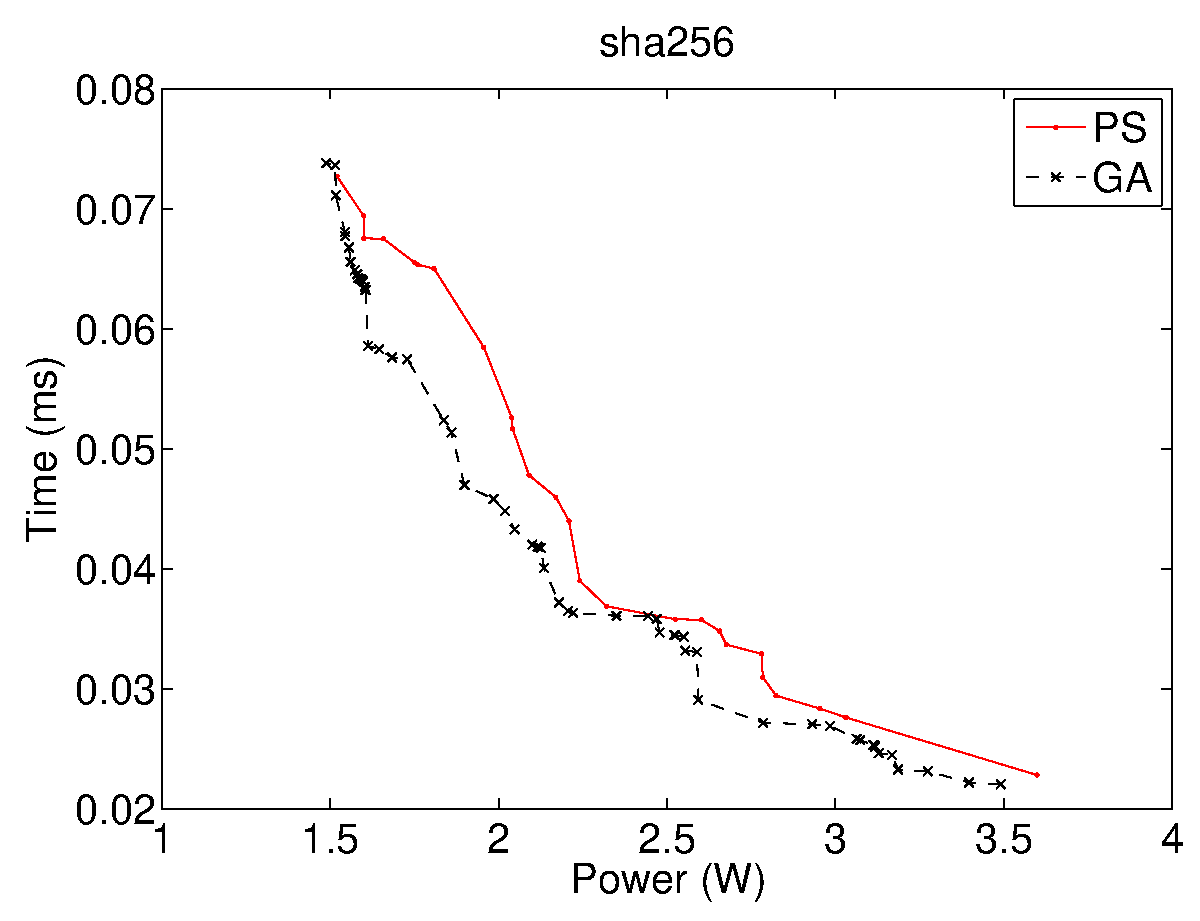
\includegraphics[width=0.30\textwidth]{pictures/sha_500_bis.eps}
    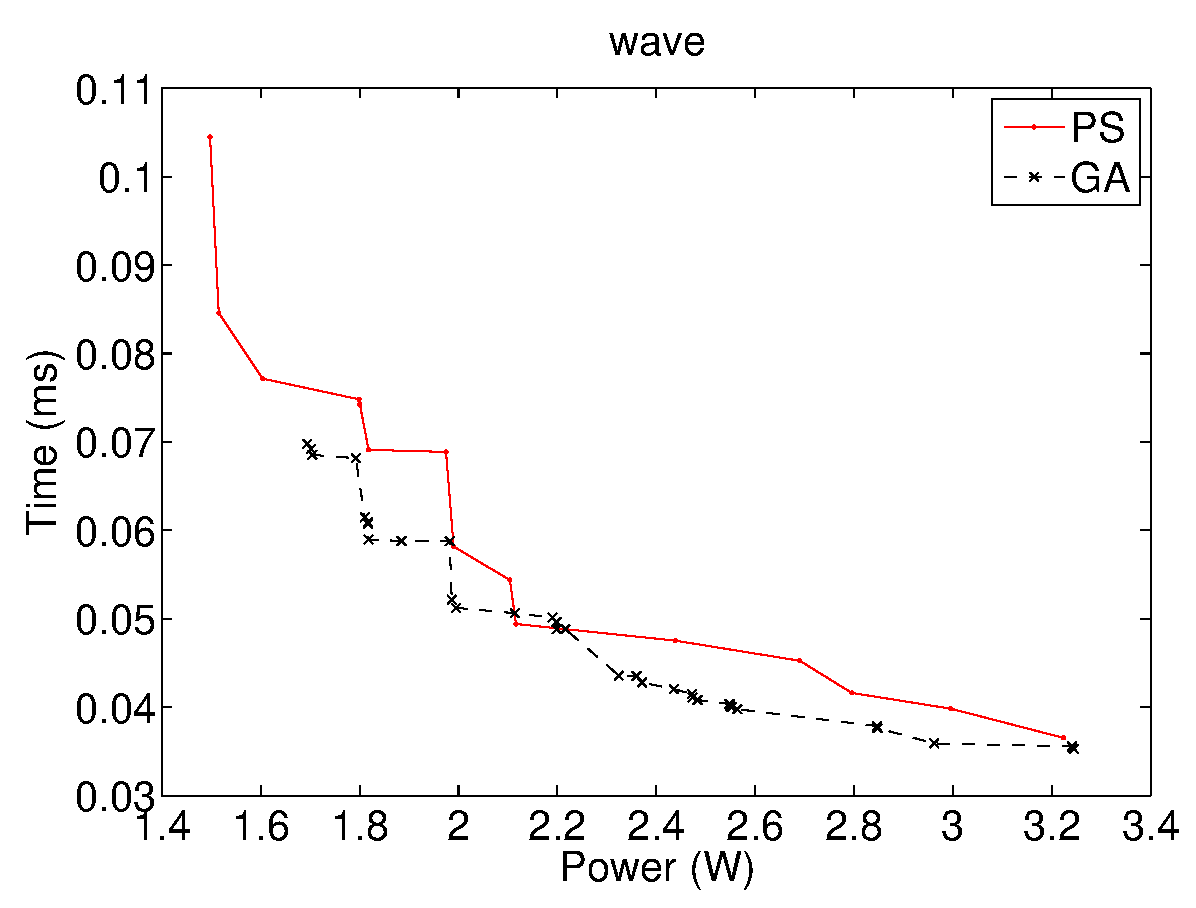
\includegraphics[width=0.30\textwidth]{pictures/wave_500.eps} 
  \end{center}
\end{figure}

Low budget Pareto sets are shown in \figR{pareto_fronts_100}. Note
that with such a small number of configurations being investigated, the
two sets are often overlapping, being also strongly dependent upon the
application being considered.  These results are obtained in about 5
eras and demonstrate that, with such a limited budget, PS can compete with
genetic approach while even discovering very different Pareto fronts.
Considering the extended simulation budget as depicted in
\figR{pareto_fronts_500}, we can qualitatively observe that even if PS
does not strictly outperforms GA in terms of dominance, it shows
in some cases Pareto fronts whose extension is larger. We can intuitively
relate this to the ``novelty-based'' score system, so that instead of
focusing on getting better points inside a given range PS tries to
enlarge the range itself, resulting in less dense but more extended
Pareto fronts. Of course we cannot classify this different behavior as
being strictly better or worse when compared to the genetic one: other
design factors should be evaluated on a case-by-case basis, e.g. the
desired granularity of the results, objective range constraints or
estimated error of the adopted models.

To better evaluate results from a different perspective, we
adopt the \emph{variation range} and the \emph{average absolute
dispersion error}, the two quantitative metrics described and motivated
in~\secR{metrics}. In particular, a comparison between the variation
ranges of both power dissipation and execution time, obtained by PS
and GA for different benchmarks, is shown in \figR{dispersion}(a) and~(b), respectively.  As it can be observed, the PS exploration provides
solutions which fall on a range that is, on average, wider than the
one provided by a GA exploration for power dissipation and execution
time, respectively.
%\begin{table}
%  \centering
%  \begin{tabular}{c}
%    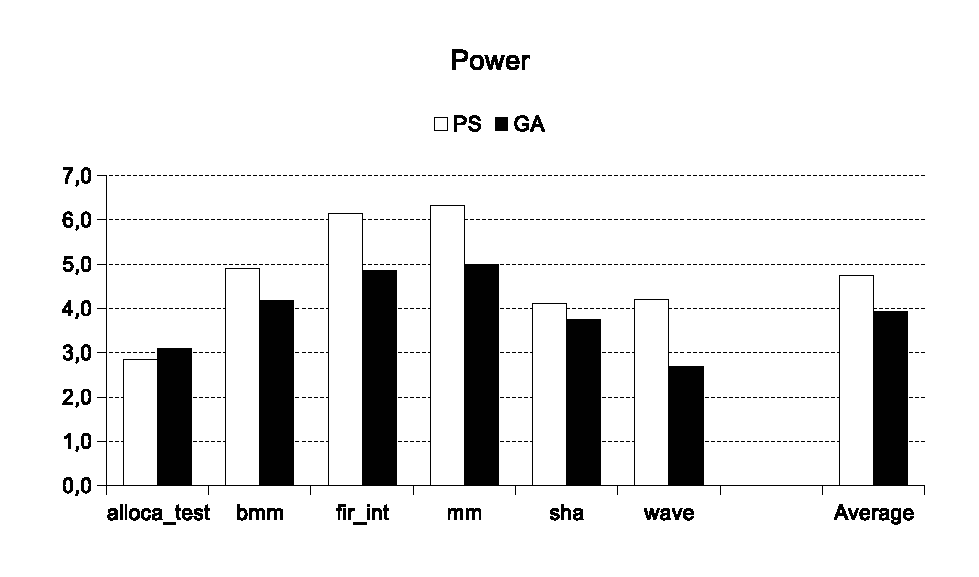
\includegraphics[width=0.7\textwidth]{pictures/variation_power.eps} \\
%    (a) \\
%    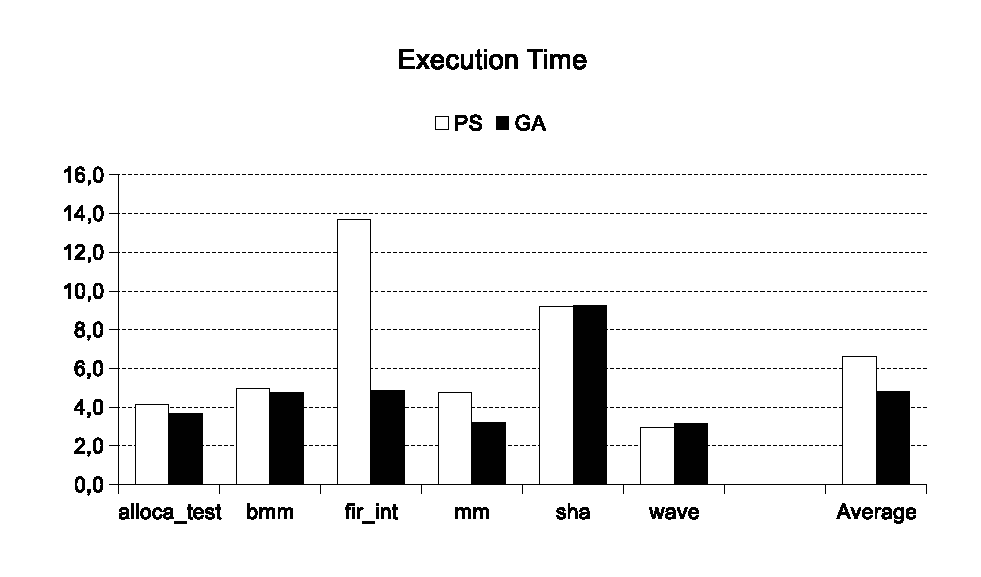
\includegraphics[width=0.7\textwidth]{pictures/variation_etime.eps} \\
%    (b) \\
%    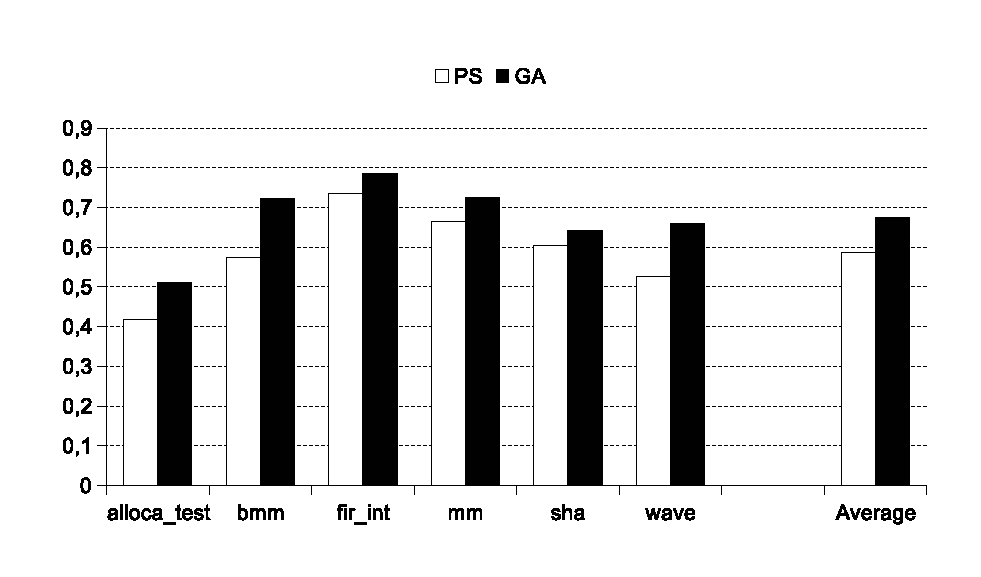
\includegraphics[width=0.7\textwidth]{pictures/dispersion.eps} \\
%    (c) 
%  \end{tabular}
%  \caption{(a)(b) Variation range obtained by PS and GA for different benchmarks
%  and average dispersion absolute dispersion (c)}
%  \label{fig:dispersion}
%\end{table}

\begin{figure}
  \figLC{dispersion}{(a)(b) Variation range obtained by PS and GA for
  different benchmarks and average absolute dispersion errors (c). }
  \begin{center}
    \subfigure[]{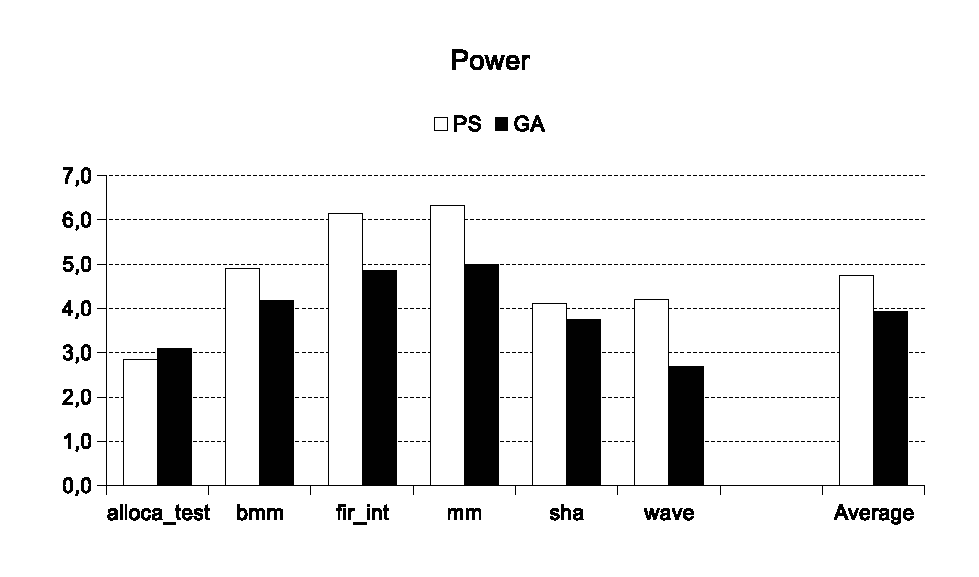
\includegraphics[width=0.7\textwidth]{pictures/variation_power.eps} }
    \subfigure[]{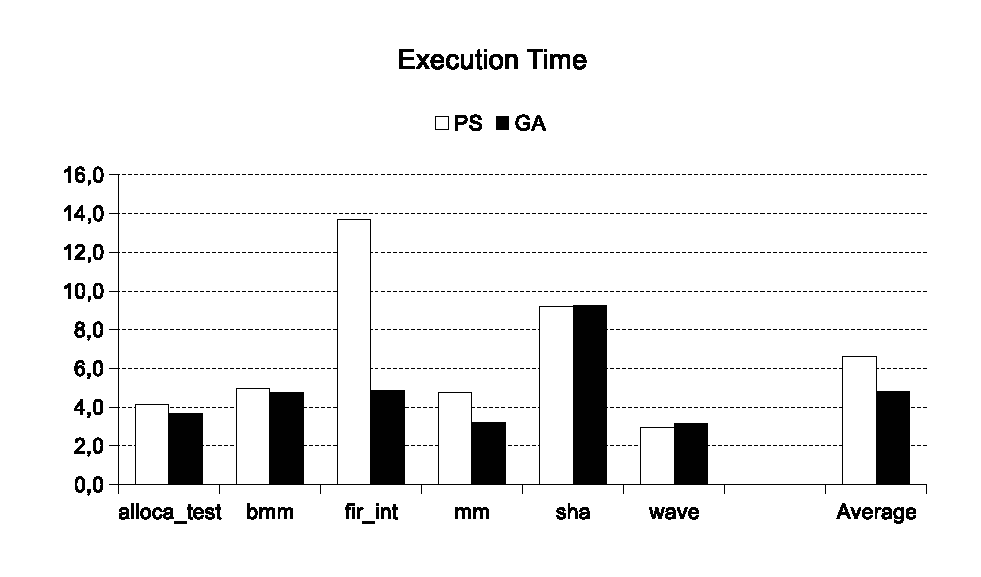
\includegraphics[width=0.7\textwidth]{pictures/variation_etime.eps} }
    \subfigure[]{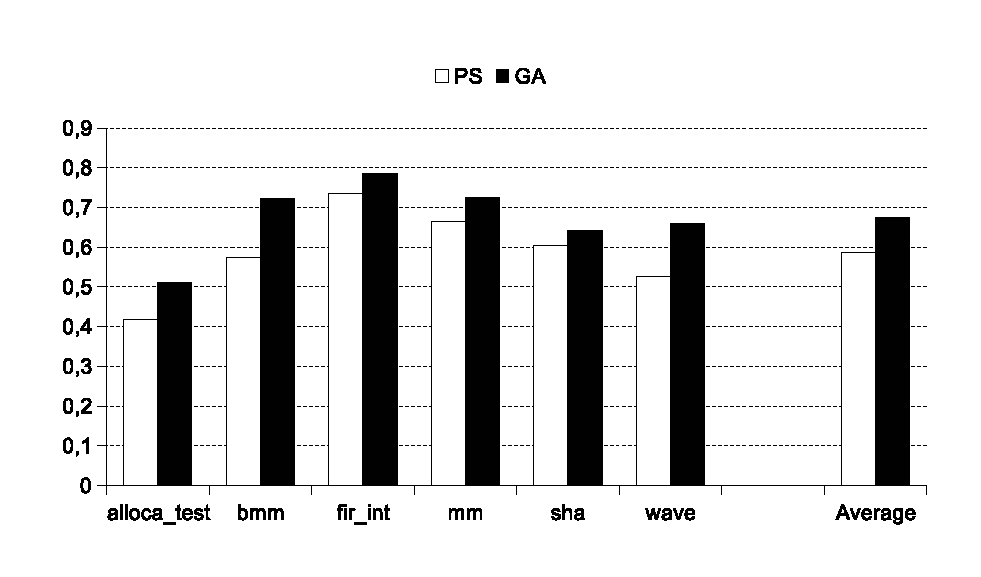
\includegraphics[width=0.7\textwidth]{pictures/dispersion.eps} }
  \end{center}
\end{figure}

\figR{dispersion}(c) shows the average normalized absolute dispersion
errors for different benchmarks for PS and GA exploration.  As it can
be observed, GA shows a tendency in discovering more uniformly
dispersed points (i.e. higher values in the chart). These results,
together with the variation ranges of \figR{dispersion}(a) and~(b)
confirm the density vs. extension trade-offs when comparing PS and
GA approaches. We highlight that PS shows a stronger \emph{uniform convergence} (discussed in \secR{metrics}), i.e. it provides a more extended Pareto front, avoiding the designer to neglect some important options, and offering a wider view of the potentials of the designed device.

Finally, it should be pointed out that the final output of PS
execution is not only the Pareto-optimal set of configurations, but also
a partitioning of the parameter space in more or less innovative
regions, obtained as a result of the merge/splitting operators
described in~\secR{algorithm}. Exploiting the information carried out
by this partitioning could be an interesting added-value of PS to be
investigated in future developments of the proposed strategy.

%Nevertheless, the proposed algorithm introduces a new
%perspective on the allocation of a simulations budget, paving the way for
%the development of further strategies for addressing the problem of
%multi-objective hardware/software design space exploration.



%------------------------------------------------------------------------------

\section{Conclusions}
In this work we presented a multiobjective strategy which 
introduces the concept of Parameter Space representation of Pareto
Front. A case study of a VLIW architecture involving strong
hardware/software dependencies has been carried out to evaluate
effectiveness with different amount of simulations budget.
A qualitative/quantitative comparison against a widespread multiobjective genetic
approach showed how the proposed strategy can result in a different
distribution of Pareto points which trades solutions granularity with
improved pareto extension. 

\balance

\bibliographystyle{ACM-Reference-Format-Journals} 
\bibliography{bibliography}

% TODO: G2012 bib not used ?

\end{document}
